\documentclass[letter,12pt]{article}

%page setup
\usepackage[utf8x]{inputenc}
\usepackage[toc,page]{appendix}
\usepackage[margin=1in]{geometry}
\usepackage{indentfirst}
\usepackage{setspace}
\usepackage{fancyhdr}

%for graphics handling
\usepackage{graphicx}
\usepackage{epstopdf}
%\usepackage{float}

%for math
\usepackage{mathtools}
\usepackage{mathrsfs}
\usepackage{gensymb} 
\usepackage{amsmath}

%for references
%\usepackage{natbib}
\usepackage{authblk} 

%for typesetting
\usepackage{color}
\usepackage{ulem}
\usepackage{listings}
\usepackage{lineno}
\usepackage{hyperref}
\usepackage{courier}



%opening
\title{\vspace{-2.0cm}ARAFE Build and Test Manual}
\author[1]{Brian Clark \thanks{clark.2668@osu.edu}}
\author[1]{Patrick Allison \thanks{allison.122@osu.edu}}
%\author[1]{Suren Gourapura \thanks{gourapura.2@osu.edu}}
%\author[1]{Lucas Smith \thanks{smith.10444@osu.edu}}
\affil[1]{\footnotesize{Department of Physics \& Center for Cosmology and Astroparticle Physics (CCAPP), The Ohio State University}}

\begin{document}

\maketitle

\begin{abstract}
In this document we will detail the procuedure for testing and debugging the ARA Advanced Front End (ARAFE). This includes the Power and Control (PC) boards and their associated DC-to-DC converters, as well as the Radio Frequency (RF) boards. We will describe how to test them as they are built to ensure they are functioning properly, give example oscilloscope and network analyzer traces of boards which are working correctly, as well as offer practical debugging advice as the boards are built. Finally, we detail a procedure for how the RF board s-parameter files should be measured and named, and also describe where they are stored in the data warehouse, which will be of use to data analyzers and simulators.
\end{abstract}

\tableofcontents
\newpage

\section{General Comments}

\subsection{Introduction}

A completed ARAFE module, or ARAFE quad, consists of one power and control (PC) board and one radio frequency (RF) board. Each RF board contains four channels of signal conditioning, with tunable attenuation for signal and trigger paths. As such, there are four quads per station for all sixteen antennas. The four quads are controlled by one ARAFE master board. Therefore, a complete ARAFE system consists of four PC boards, four RF boards, and 1 master board.

\subsection{Powering and Communicating with the Tester Boards \label{subsec:Powering-and-Communicating-Tester}}

Testing of the PC and RF board should be done with the ARAFE slave tester, which is the custom red ``MSP430 Comms Test'' board in figure \ref{comms-tester}. The communications tester provides power to the quad, and also provides communications-over-power, as detailed \href{https://www.dropbox.com/s/eggk51tj8gkmlpj/arafe_master_stuff.pdf?dl=0}{here} and originally \href{http://electronicdesign.com/communications/simple-circuit-communicates-over-low-voltage-power-lines}{here}. So, the comms-tester powers and talks to the ARAFE quads. Communication to the comms-tester is provided by a custom built USB-to-UART converter, the blue board in figure \ref{USB-to-UART}. The comms-tester and USB-to-UART bords can be plugged in to one another as in figure \ref{CommsTester_and_USBtoUART}. 

Power is delivered to the comms tester by providing a 15V rail and GND to J4. Power is provided from the comms-tester to the quads by the SMA output, or J1. Communication from laptop to the USB-to-UART bridge is provided by the mini-USB port, or J1. All of this can be seen in the functional diagram in the top of figure \ref{CommsTester_and_USBtoUART}.

\begin{figure}
\begin{centering}
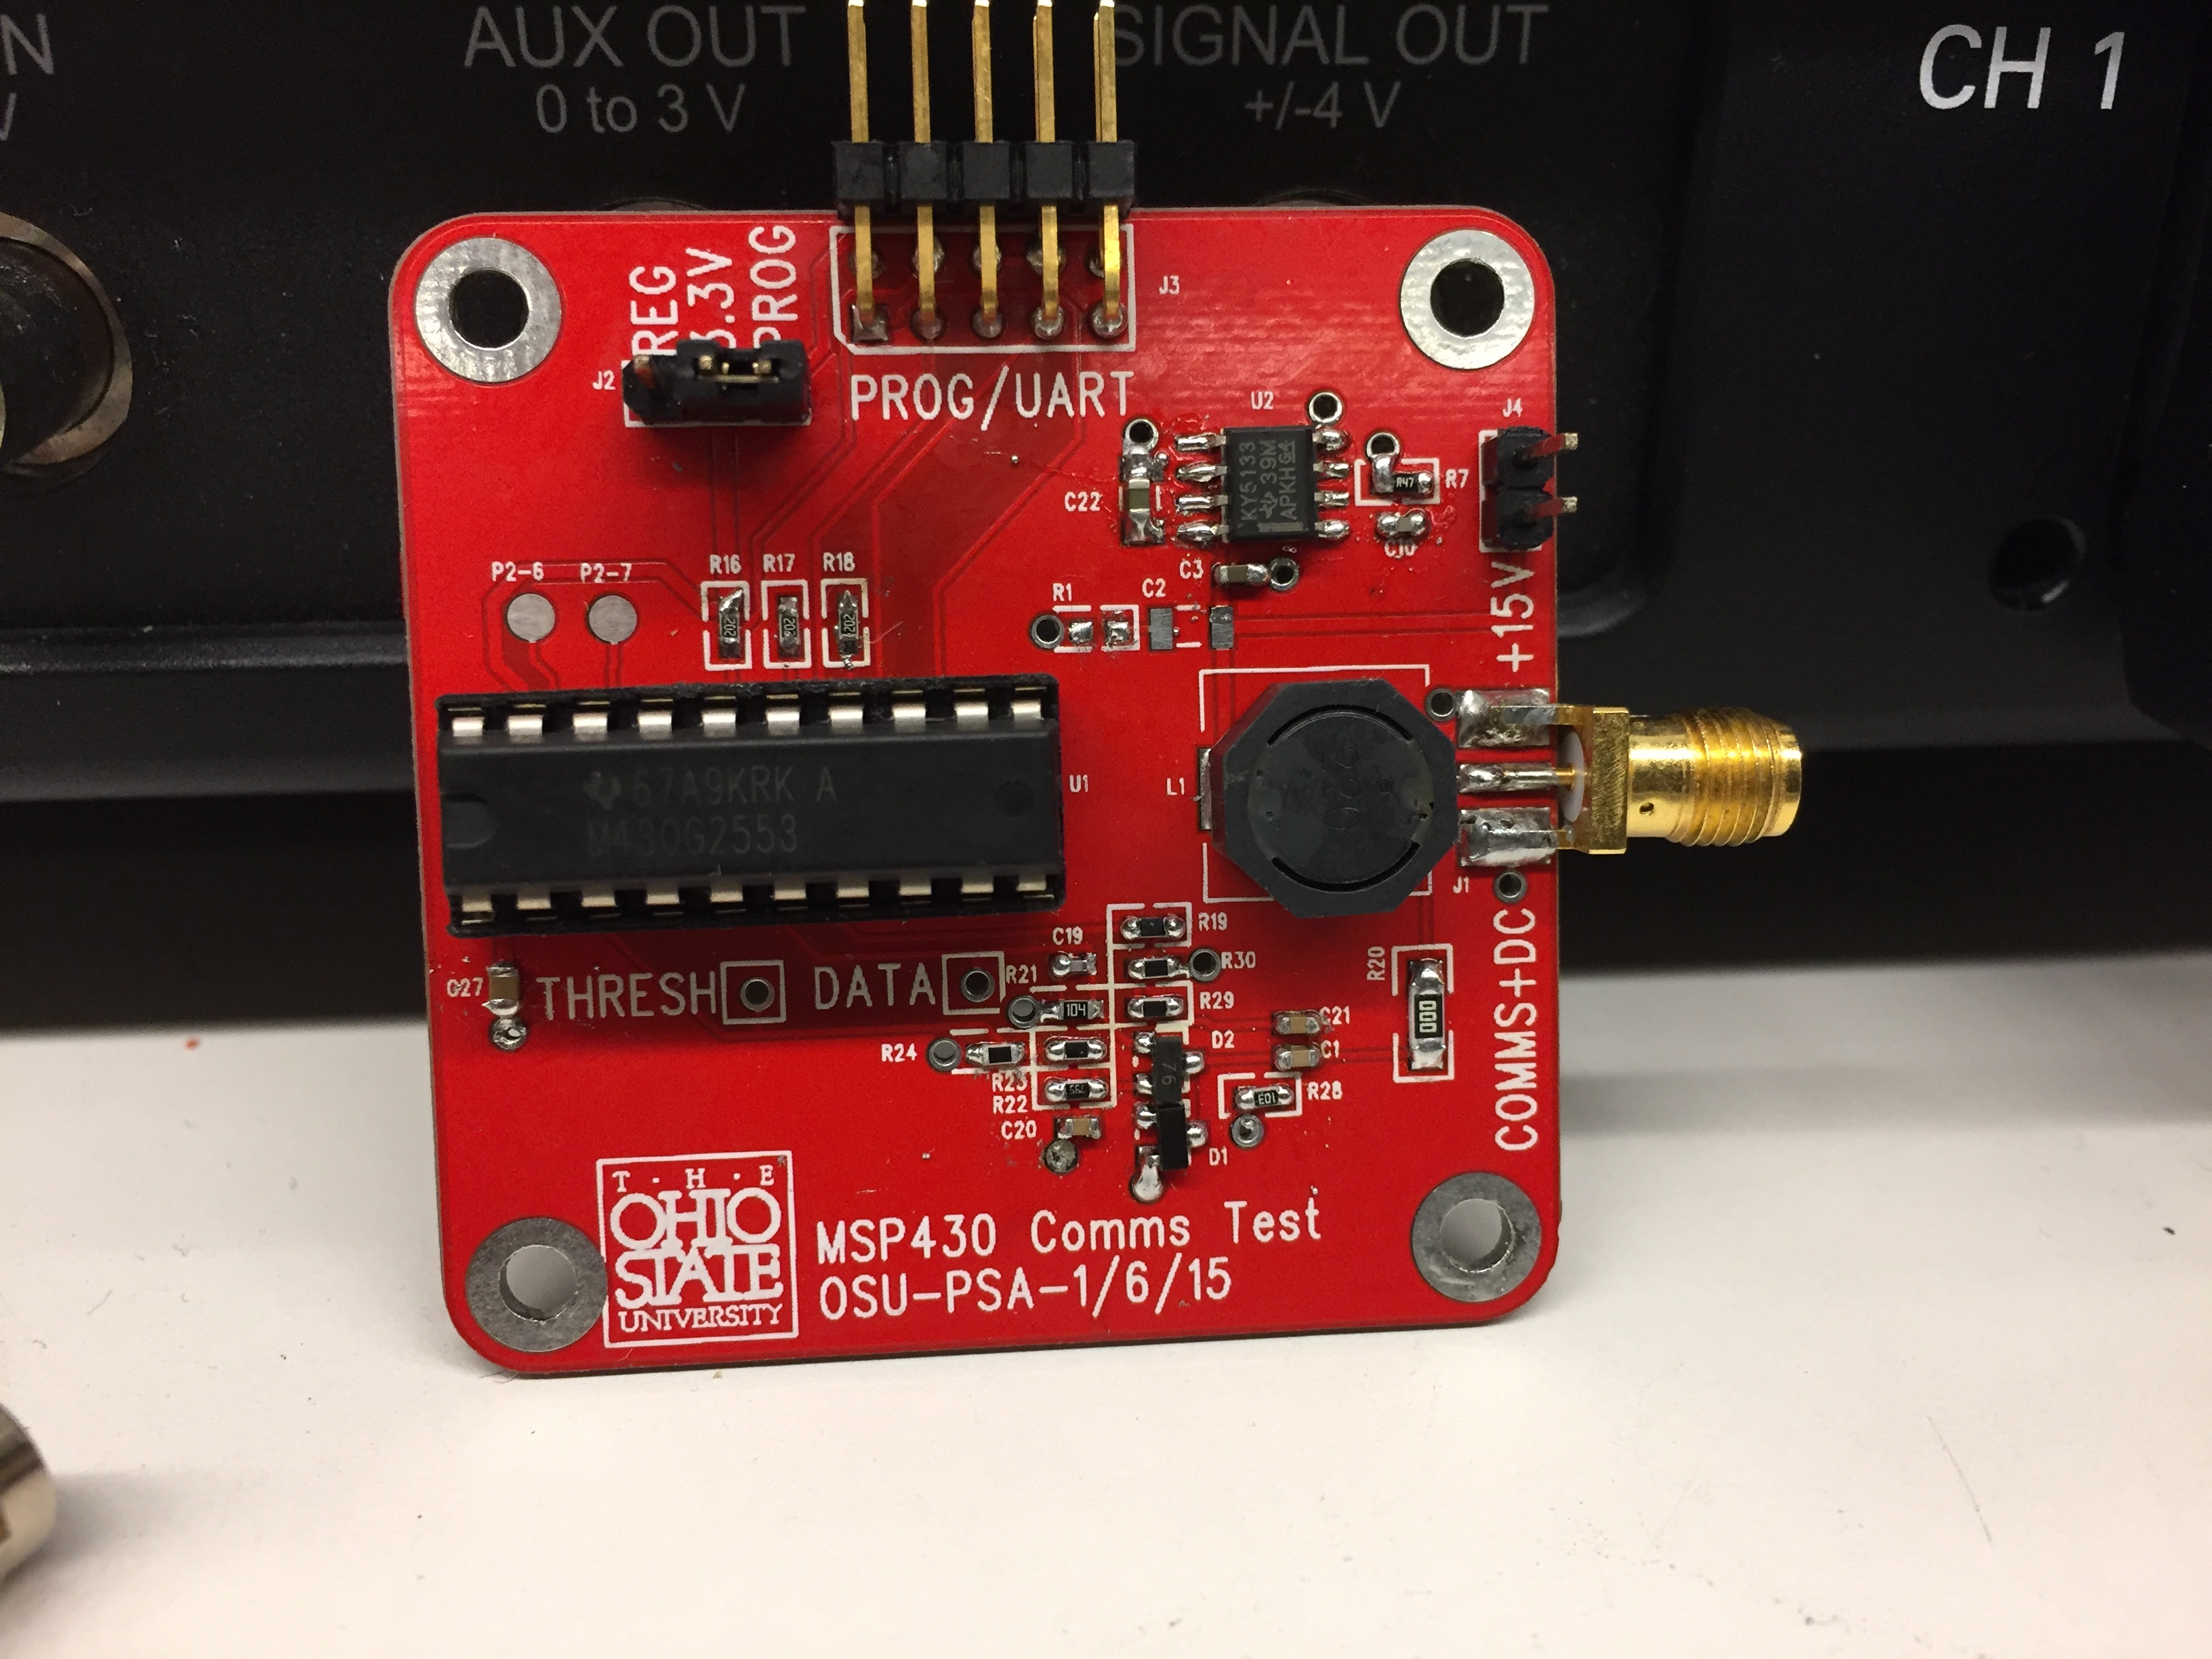
\includegraphics[width=0.5\textwidth]{photos/MS430_CommsTester.jpg}
\par\end{centering}
\caption{A photo of the MSP 430 Comms Tester. This board serves as a master
to the PC slaves. }
\label{comms-tester}
\end{figure}

\begin{figure}
\begin{centering}
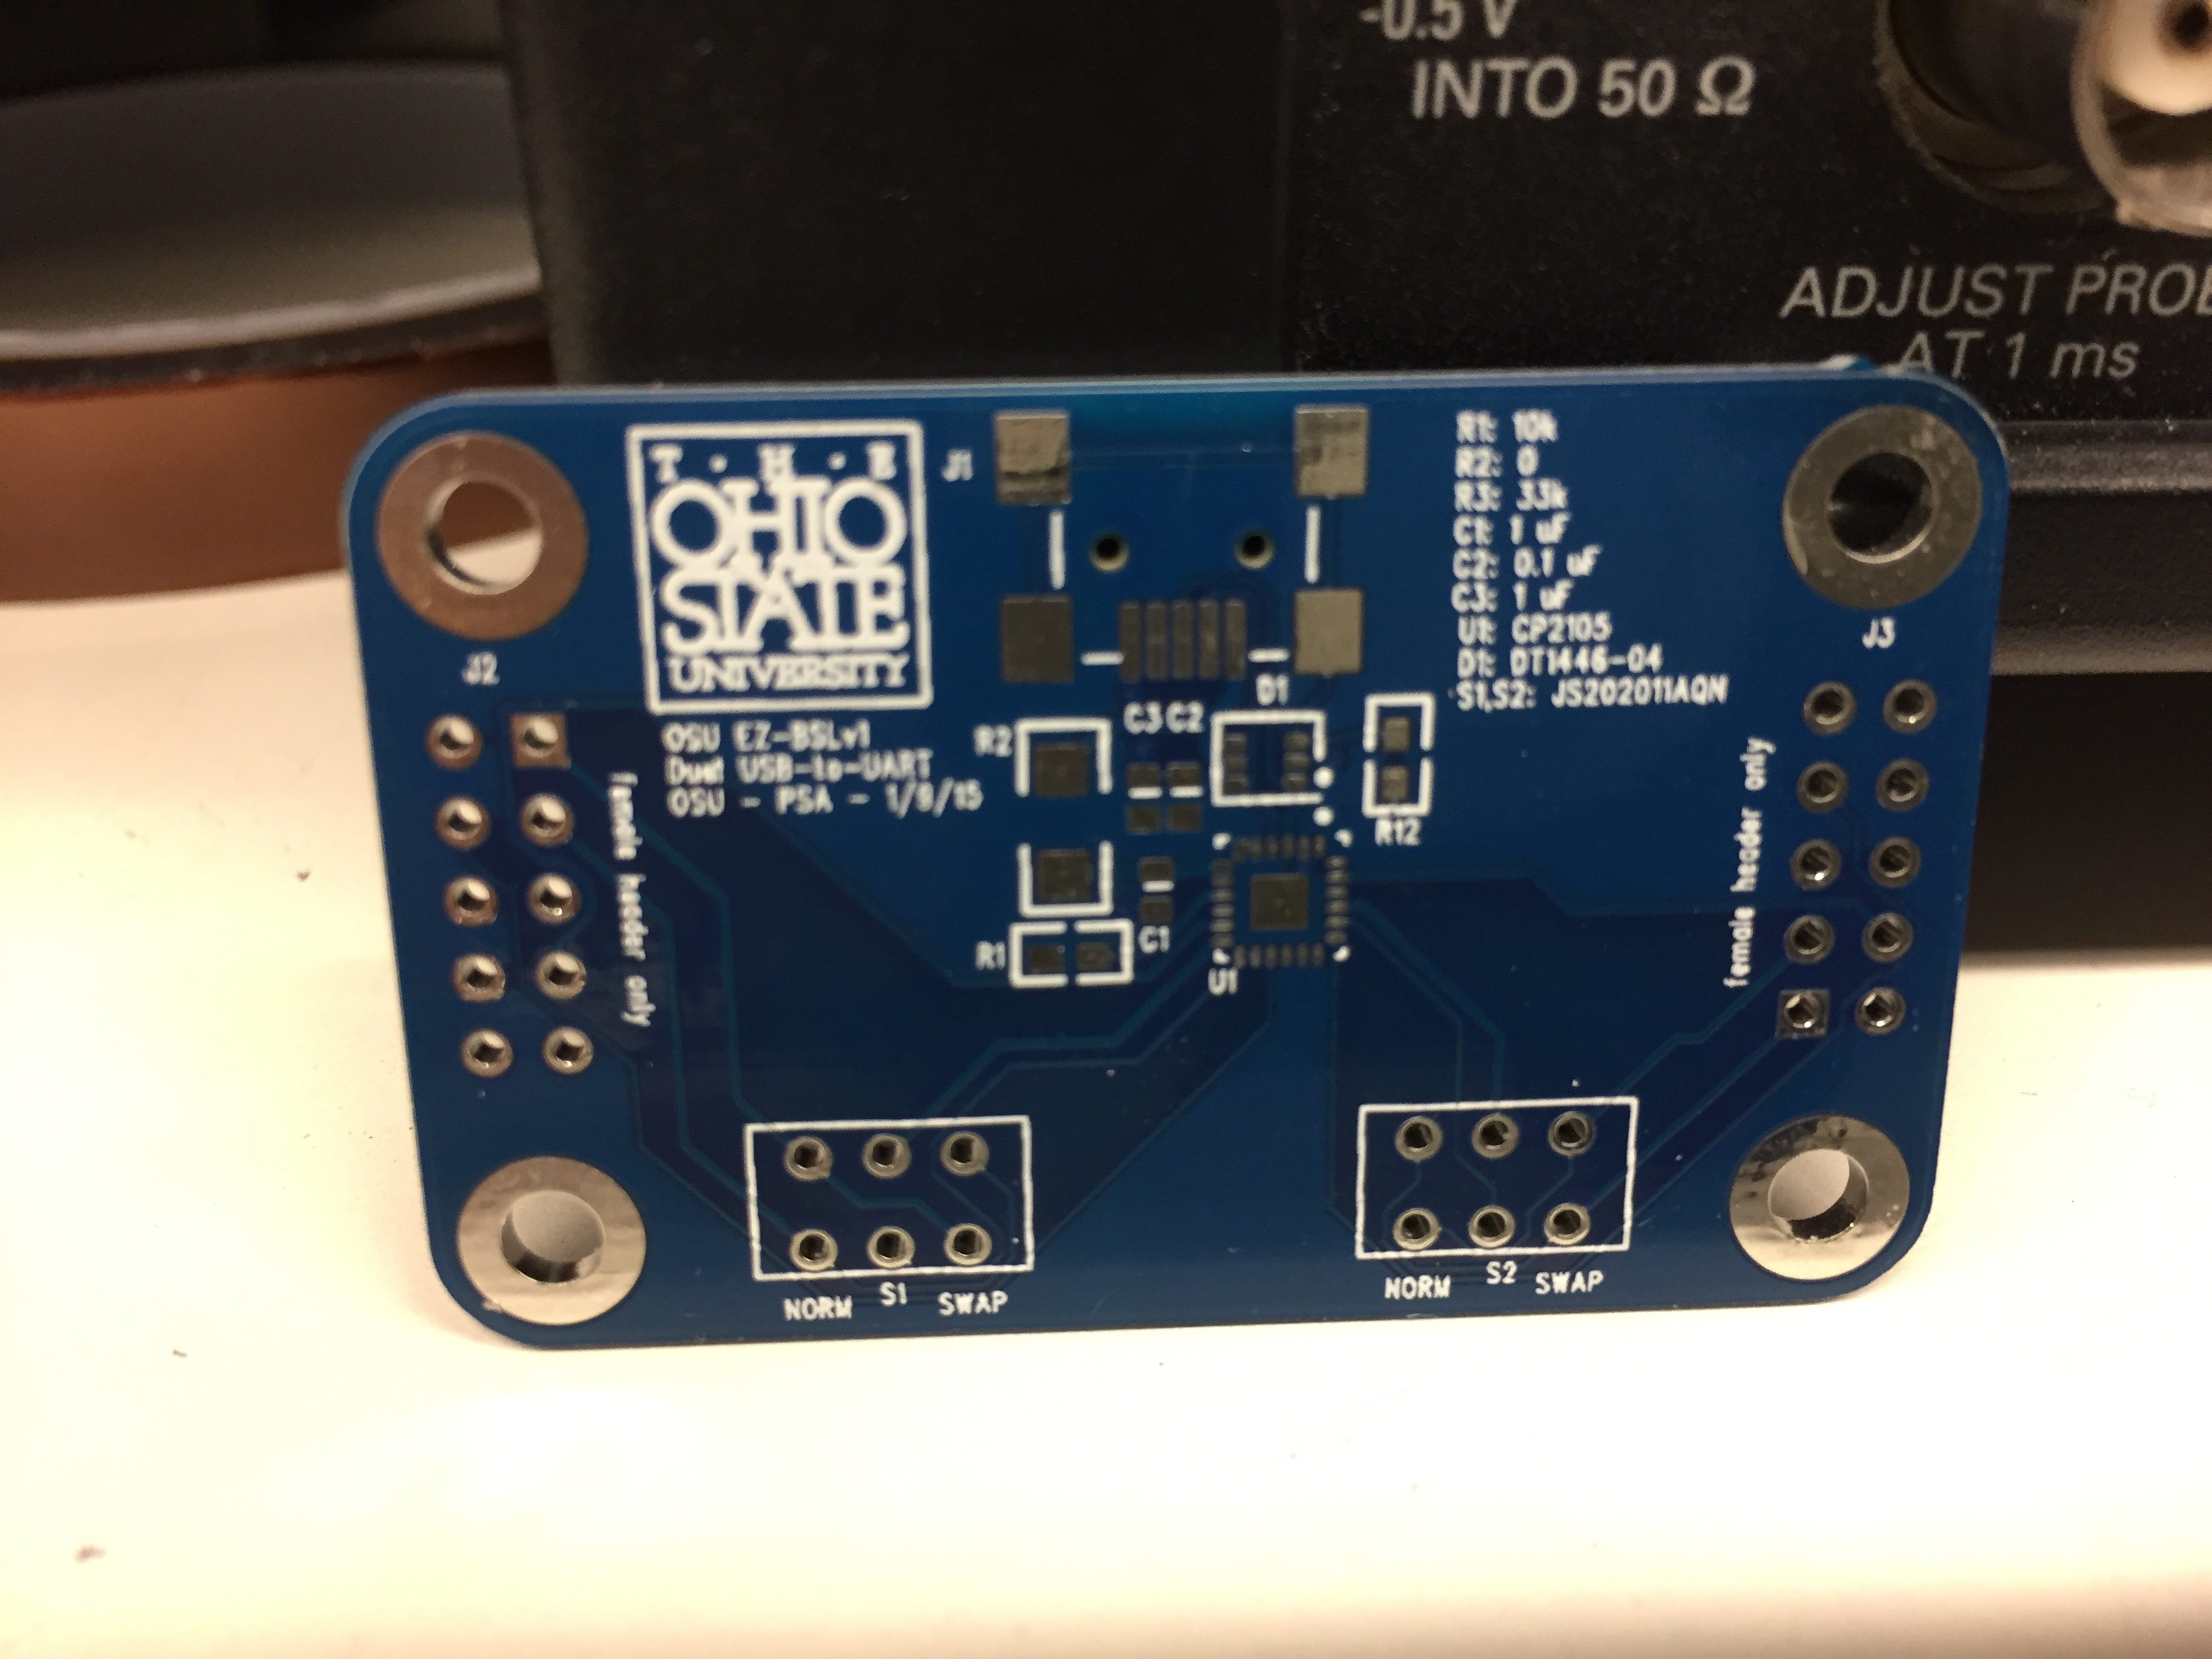
\includegraphics[width=0.5\textwidth]{photos/USB-to-UART.jpg}
\par\end{centering}
\caption{A photo of the USB-to-UART converter. This board serves as a USB interface
between a computer (like a laptop) and the MSP430 Comms Tester.}
\label{USB-to-UART}
\end{figure}

\begin{figure}
\begin{centering}
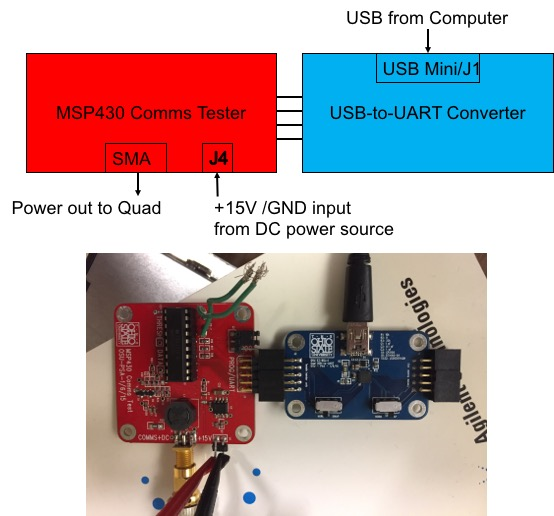
\includegraphics[width=0.75\textwidth]{photos/CommsTester_and_USBtoUART-Diagram.jpg}
\par\end{centering}
\caption{A photo of how to connect the MSP430 Comms Tester to the USB-to-UART
converter, along with a functional diagram.}
\label{CommsTester_and_USBtoUART}
\end{figure}

\subsection{Powering and Communicating with the PC Boards}

The PC boards are powered by +15V and GND, delivered to J1. The two left pins are power, and the two right pins are GND. A photo of a correct powered board can be viewed in figure \ref{correct-power-PC}. The board can be powered either by the comms-tester described in section \ref{subsec:Powering-and-Communicating-Tester}, or can be powered directly by a DC power source.

Since the PC board contains a microcontroller (more on that later), it is equipped with two powering modes, controlled by the jumper J2. The orientation of the jumper J2 controls whether board is in ``program'' mode, for programming the microcontroller via TI Code-Composer studio/ MSP430 FET Pro LITE, or in ``external power'' mode, for testing with external power. When the left and middle pins of J2 are connected, the board is configured for external power. When the right and middle pins of J2 are connected, the board is configured for programming. The general procedure for powering the PC boards externally is the following:

\begin{enumerate}
\item Jumper together the leftmost pins of J2 on the PC board (the jumper setting for ``powered externally'').
\item Plug the USB-to-UART converter into the comms-tester. Wire the 15V intput and GND from a DC power source to the comms-tester, but do not turn the supply on yet. A photo of all devices plugged in and ready for use is given in figure \ref{PC-ready-to-test}.
\item From comms tester SMA output, deliver +15V to one of the two left pins of J1 on the PC board, and GND to one of the two right pins of J1 on the PC board. This is most easily done by splitting the SMA output to two micrograbbers.
\item Turn the power supply on. With only the PC board as a load (including DC-DC convereters) it should draw about 20 mA. (The photo in figure
\ref{PC-ready-to-test} shows larger current draw because it was powering an alternative set-up at the time.)
\end{enumerate}

The PC board is reverse bias protected, so if the board does not power up, the polarity of the input is the first thing to check. A photo of the board correctly connected is in figure \ref{correct-power-PC}. 

\begin{figure}
\begin{centering}
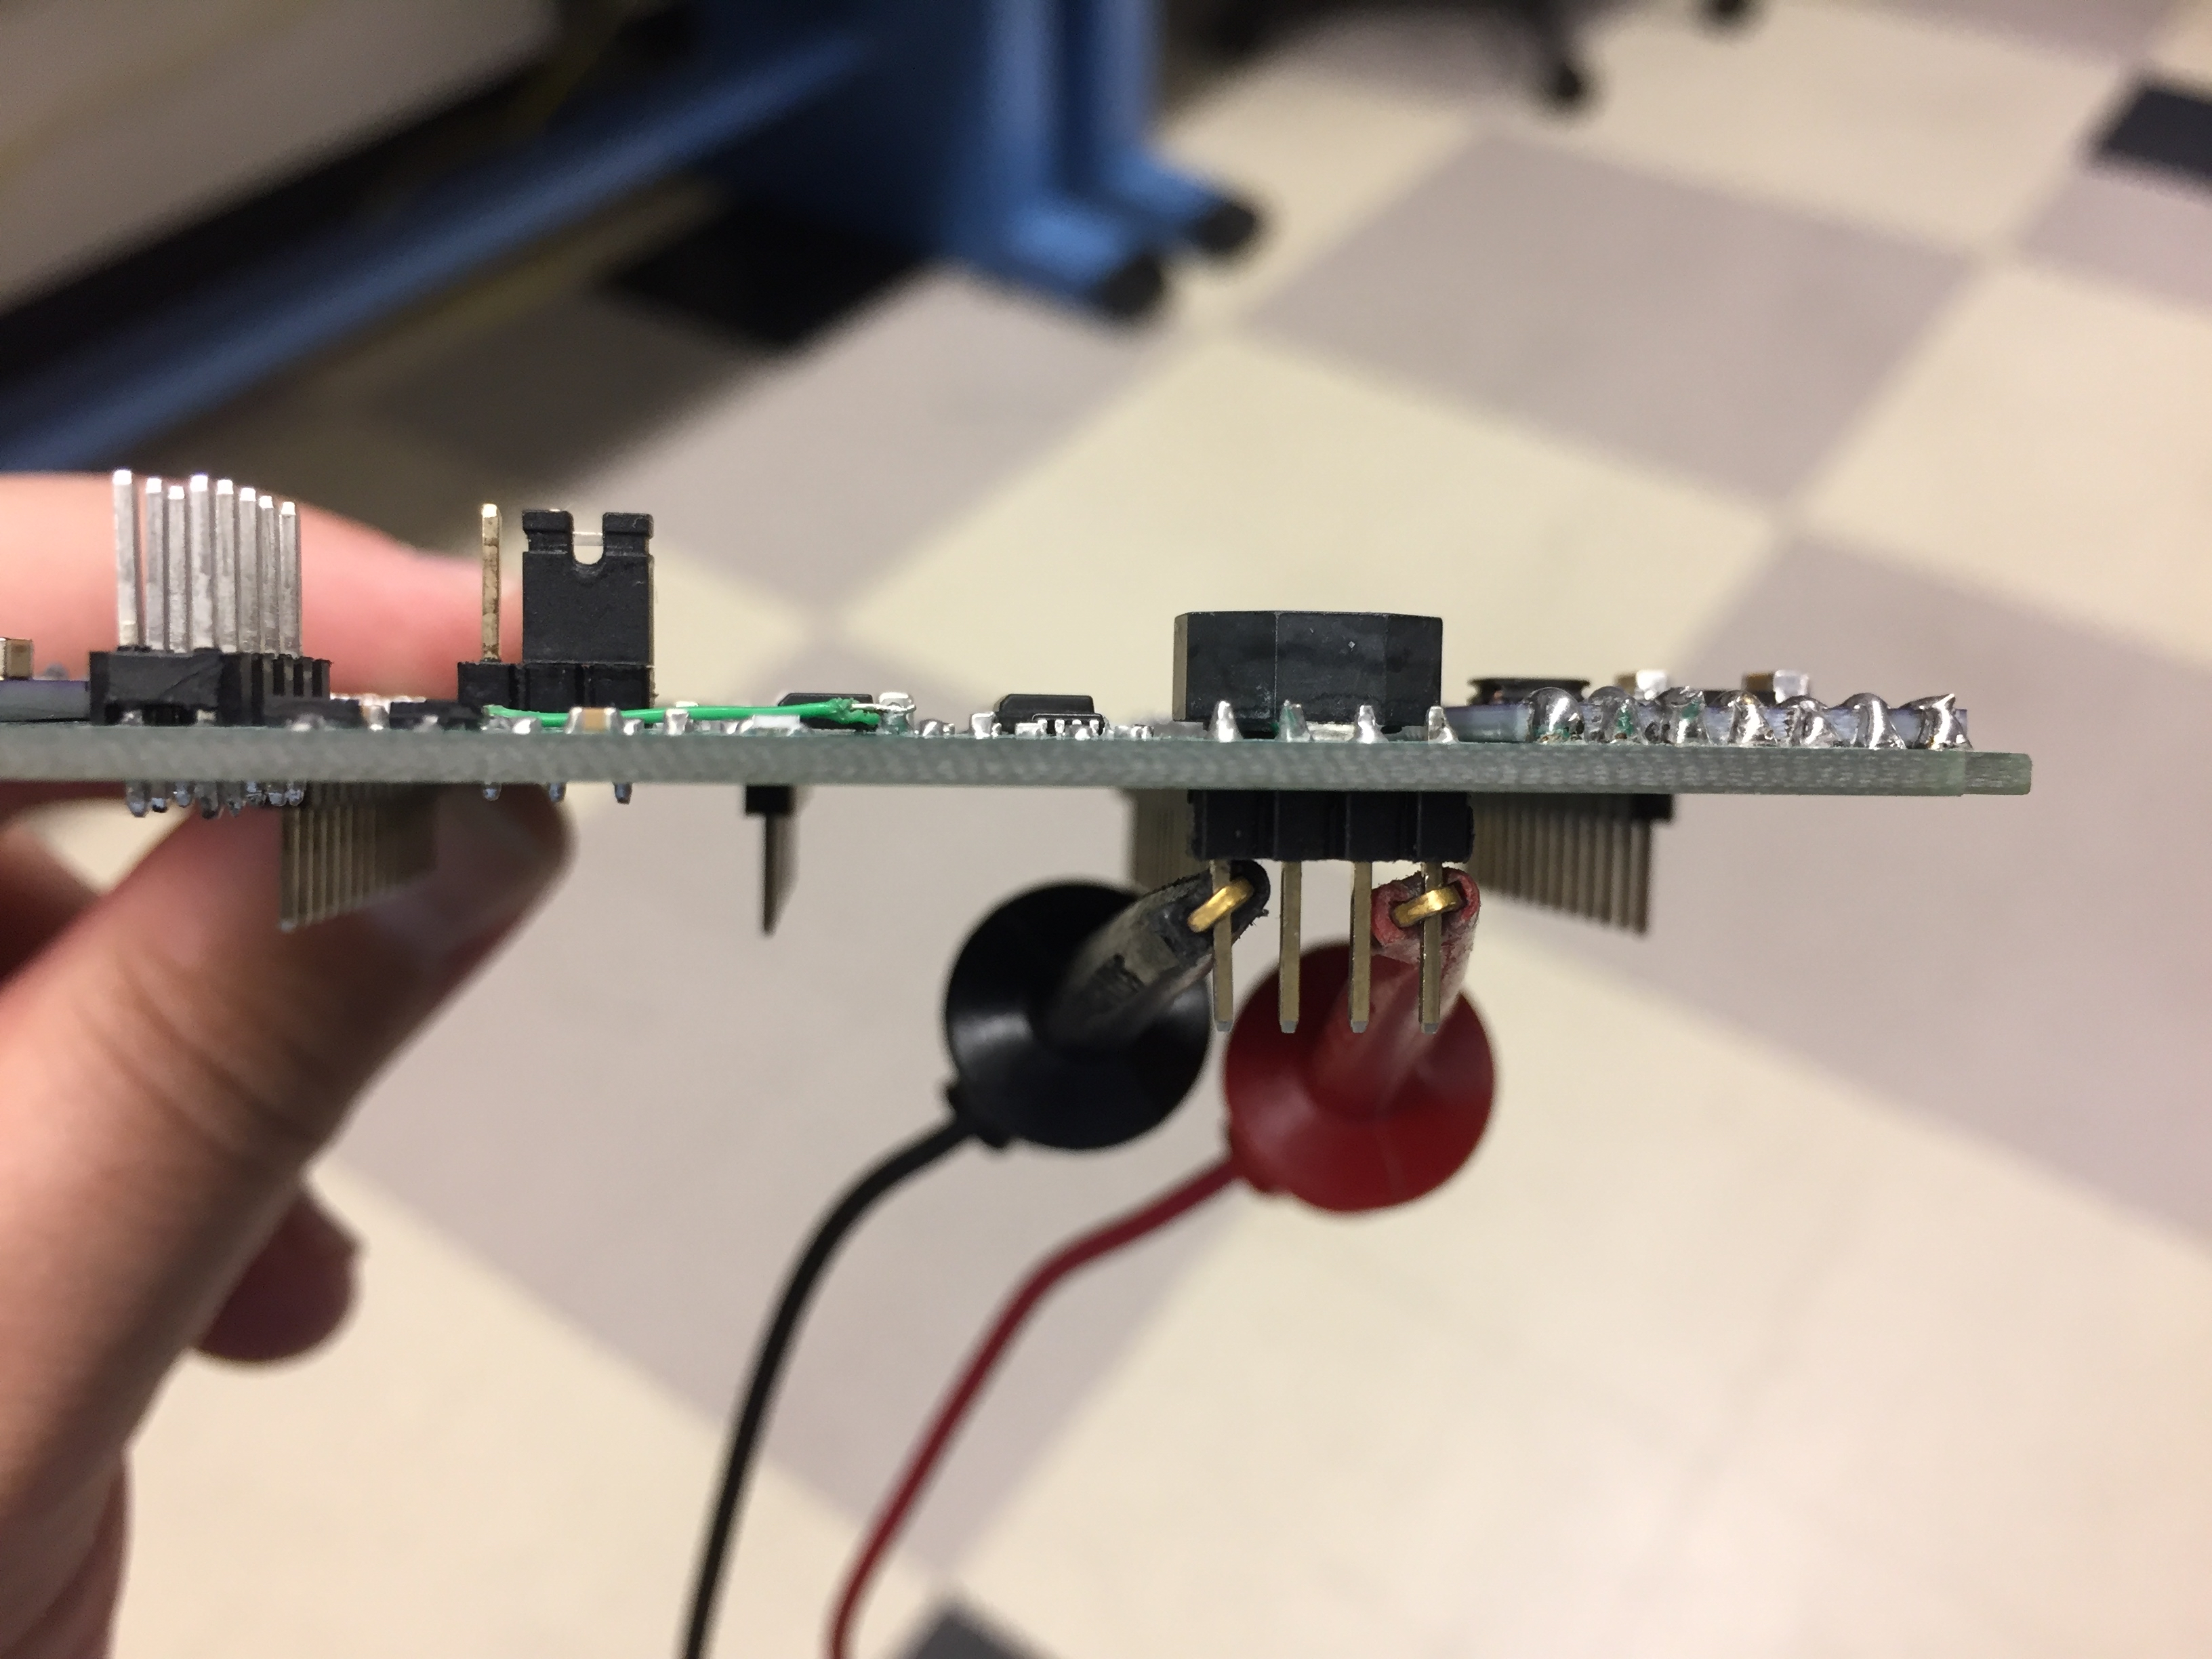
\includegraphics[width=0.75\textwidth]{photos/jumper-connection.jpg}
\par\end{centering}
\caption{A photo of a correctly powered PC board. Red is +15V and black is GND. In the upper left, you can see the left-most pins of J2 have been jumpered together for ``external power'' mode. Note that because we are looking at the board edge on from the top, ``left'' and ``right'' are mirrored relative to the text.}
\label{correct-power-PC}
\end{figure}

\begin{figure}
\begin{centering}
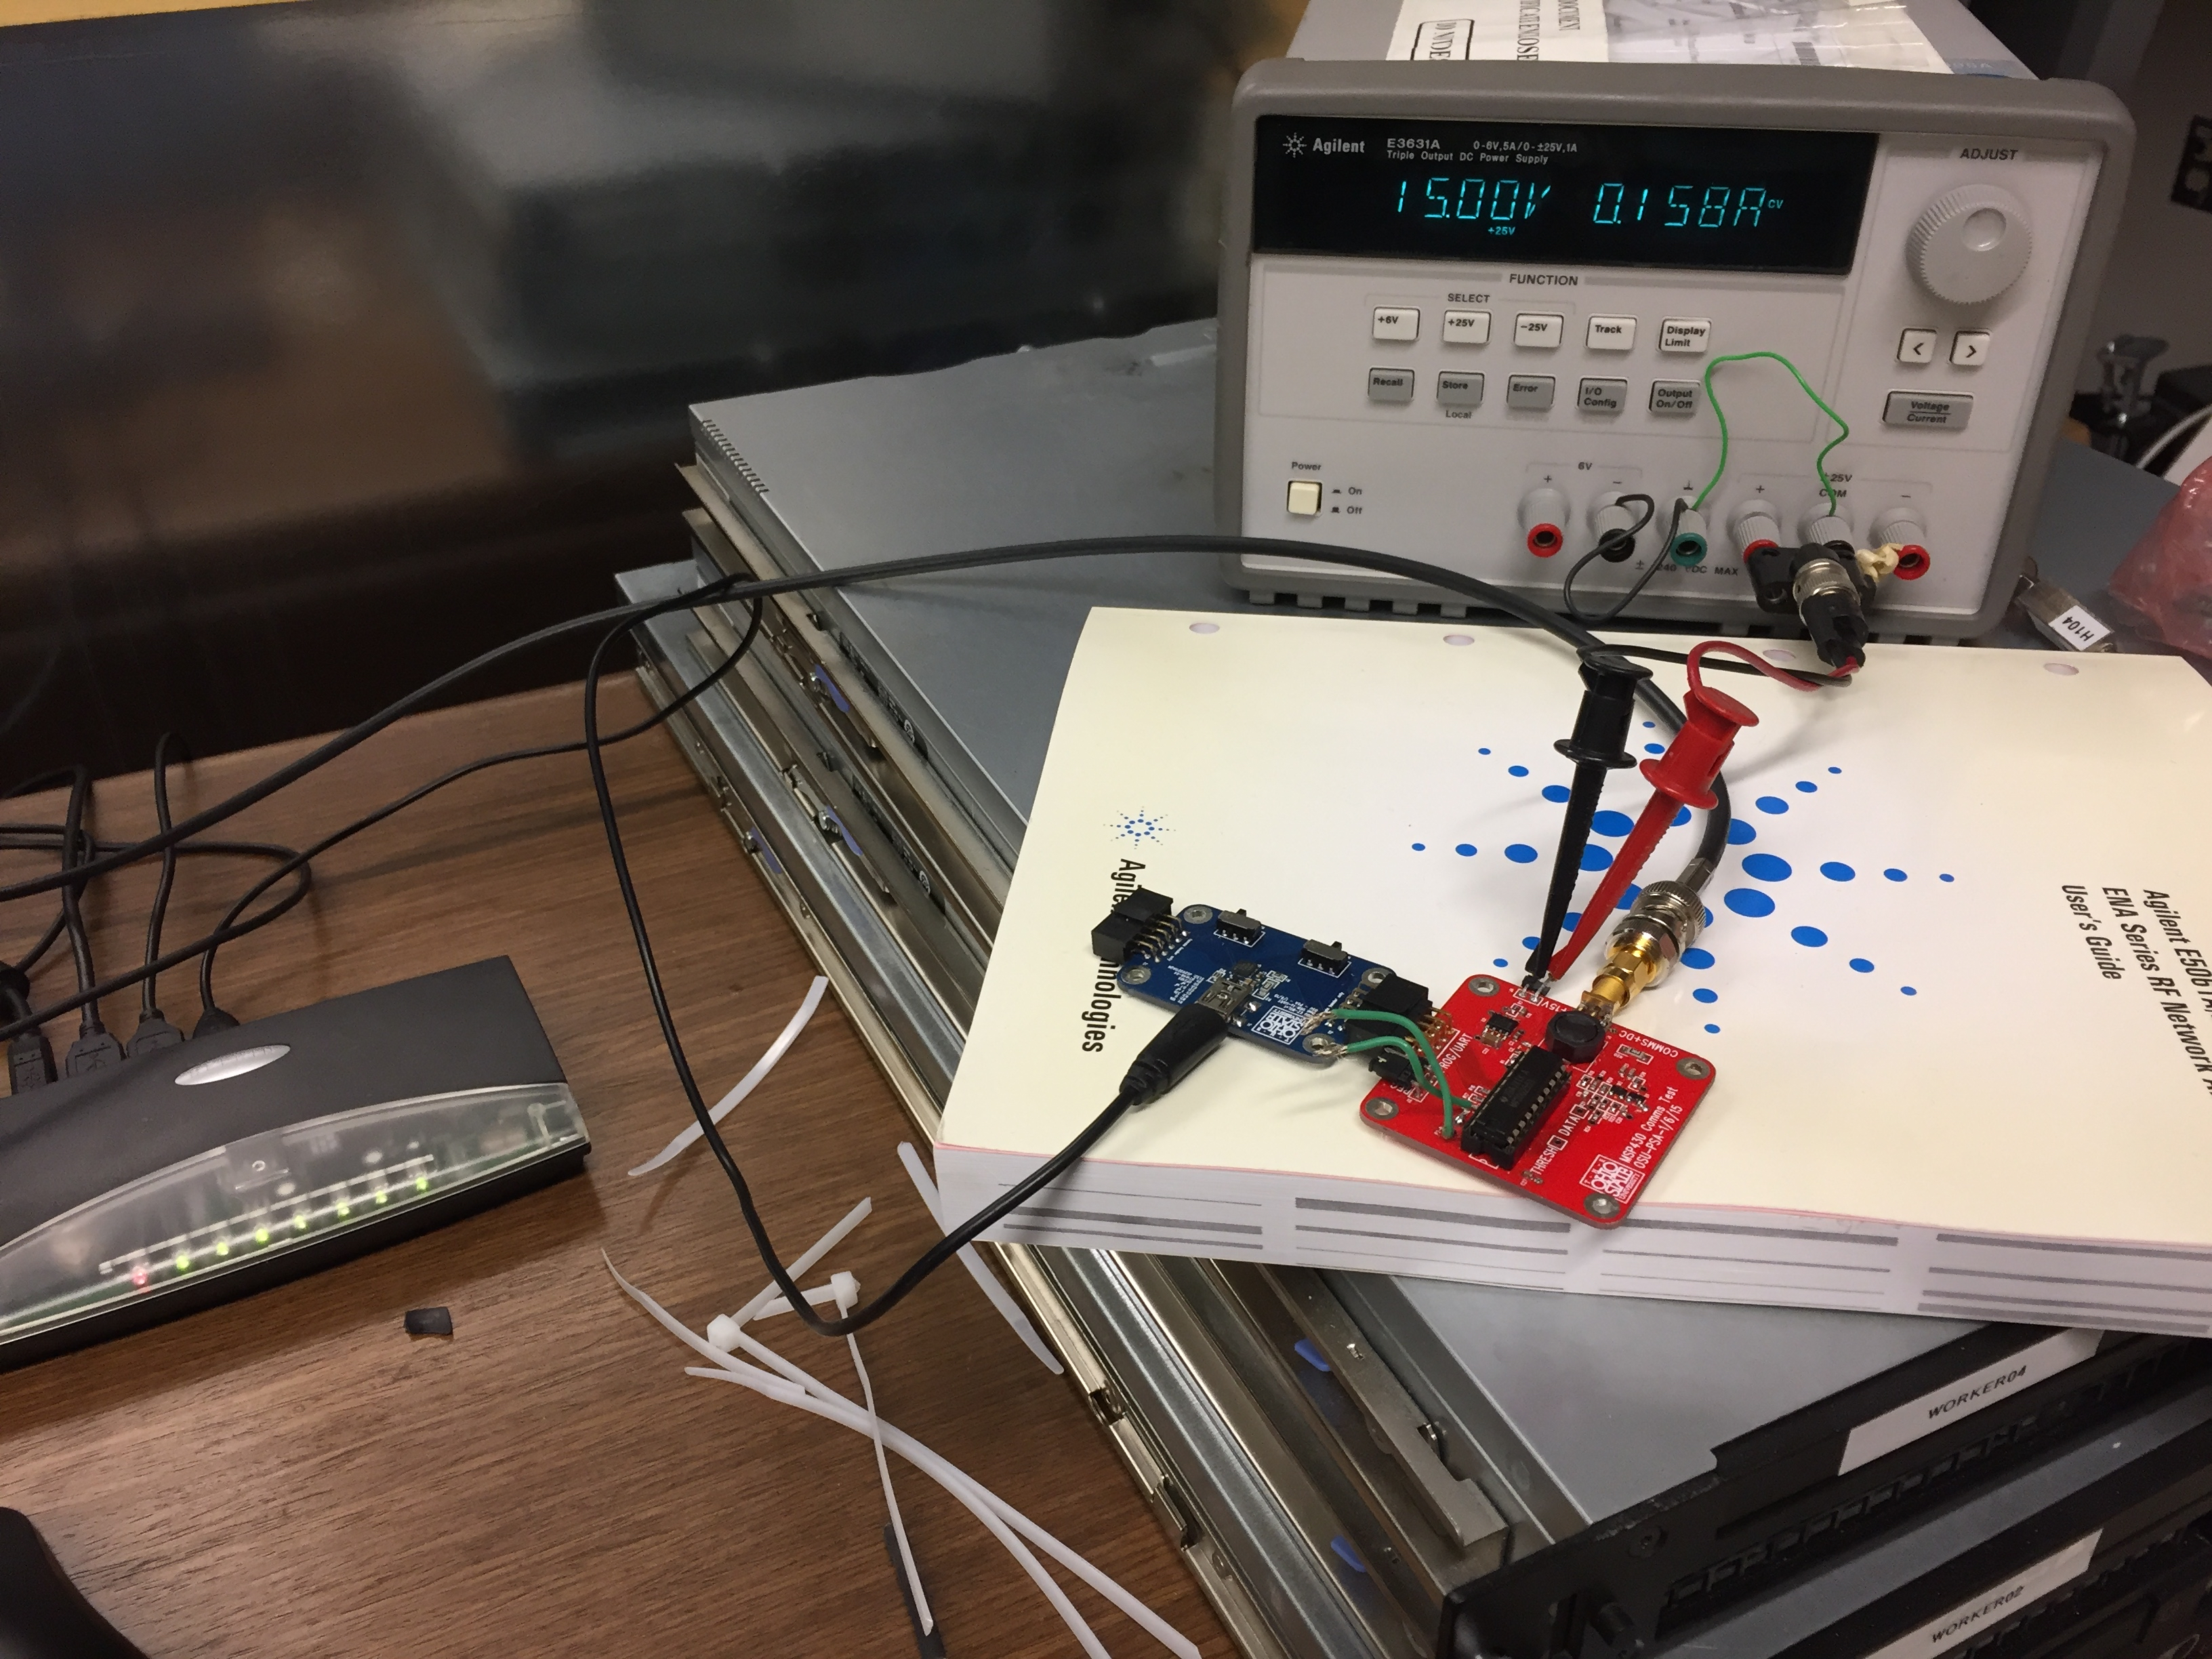
\includegraphics[width=0.75\textwidth]{photos/Power_Comms.jpg}
\par\end{centering}
\caption{A photo of the complete power supply, USB-to-UART, and MSP430 comms tester ready for testing.}
\label{PC-ready-to-test}
\end{figure}

\subsection{Powering and Communicating with the RF Boards}

Powering the RF board must be done carefully. Preferably, you should power the RF board only with the PC board, which will protect the RF board from any under/over-voltage issues, as well as reverse bias voltage. If you need to directly power an RF channel, be sure to get the polarity right, and to not apply more than +5V. Further, because the RF board is 31 mil FR4 (to keep traces thin), and because the header pins engage strongly between the PC and RF board, you should avoid plugging the PC board directly into the RF board during testing. Plying the two apart is difficult, and results in excessive flexing of the RF board. A better solution is to get a breadboard, plug in the male PC board, and wire ``arduino type'' jumper wires (eg: \href{https://www.adafruit.com/product/758}{https://www.adafruit.com/product/758}) to the female RF board. This narrower wires do not engage the female headers fully, and are much easier to remove, and even more so, can be removed without flexing the RF board. A photo of Brian Clark's test set-up in the Ohio State lab is visible in figure \ref{arafe-test-setup}.

\begin{figure}
\begin{centering}
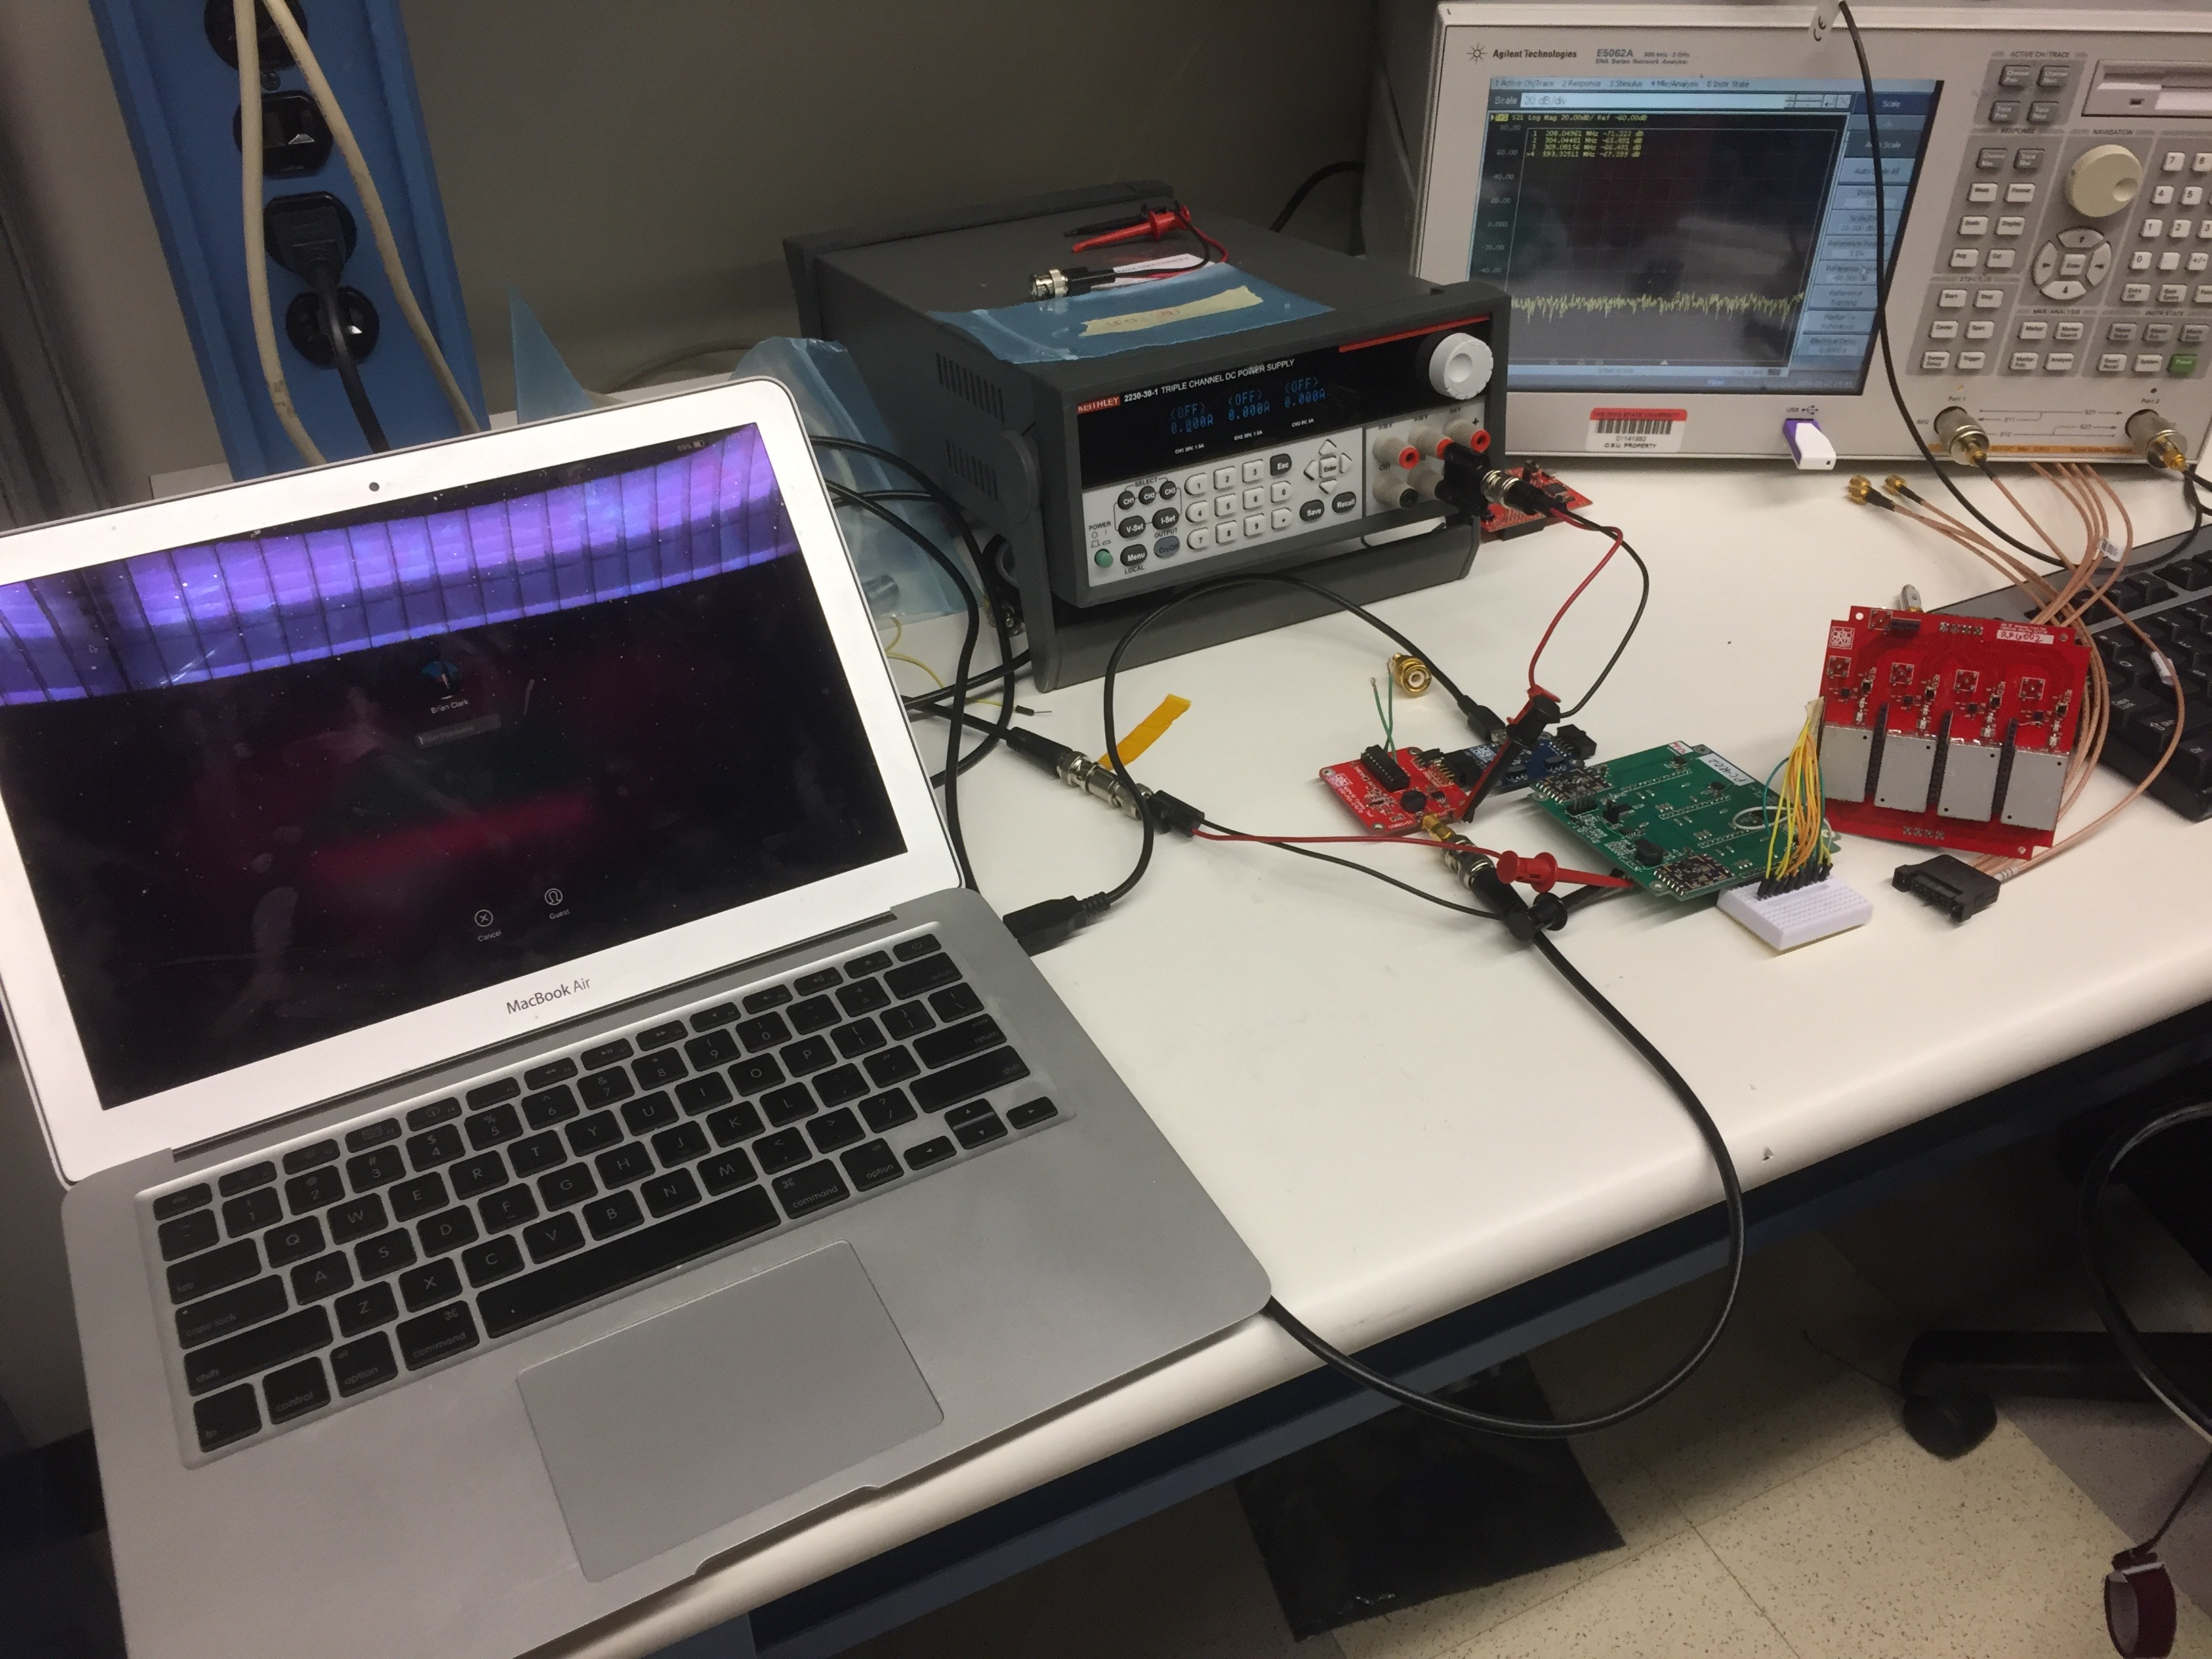
\includegraphics[width=0.5\textwidth]{photos/IMG_1212.jpg}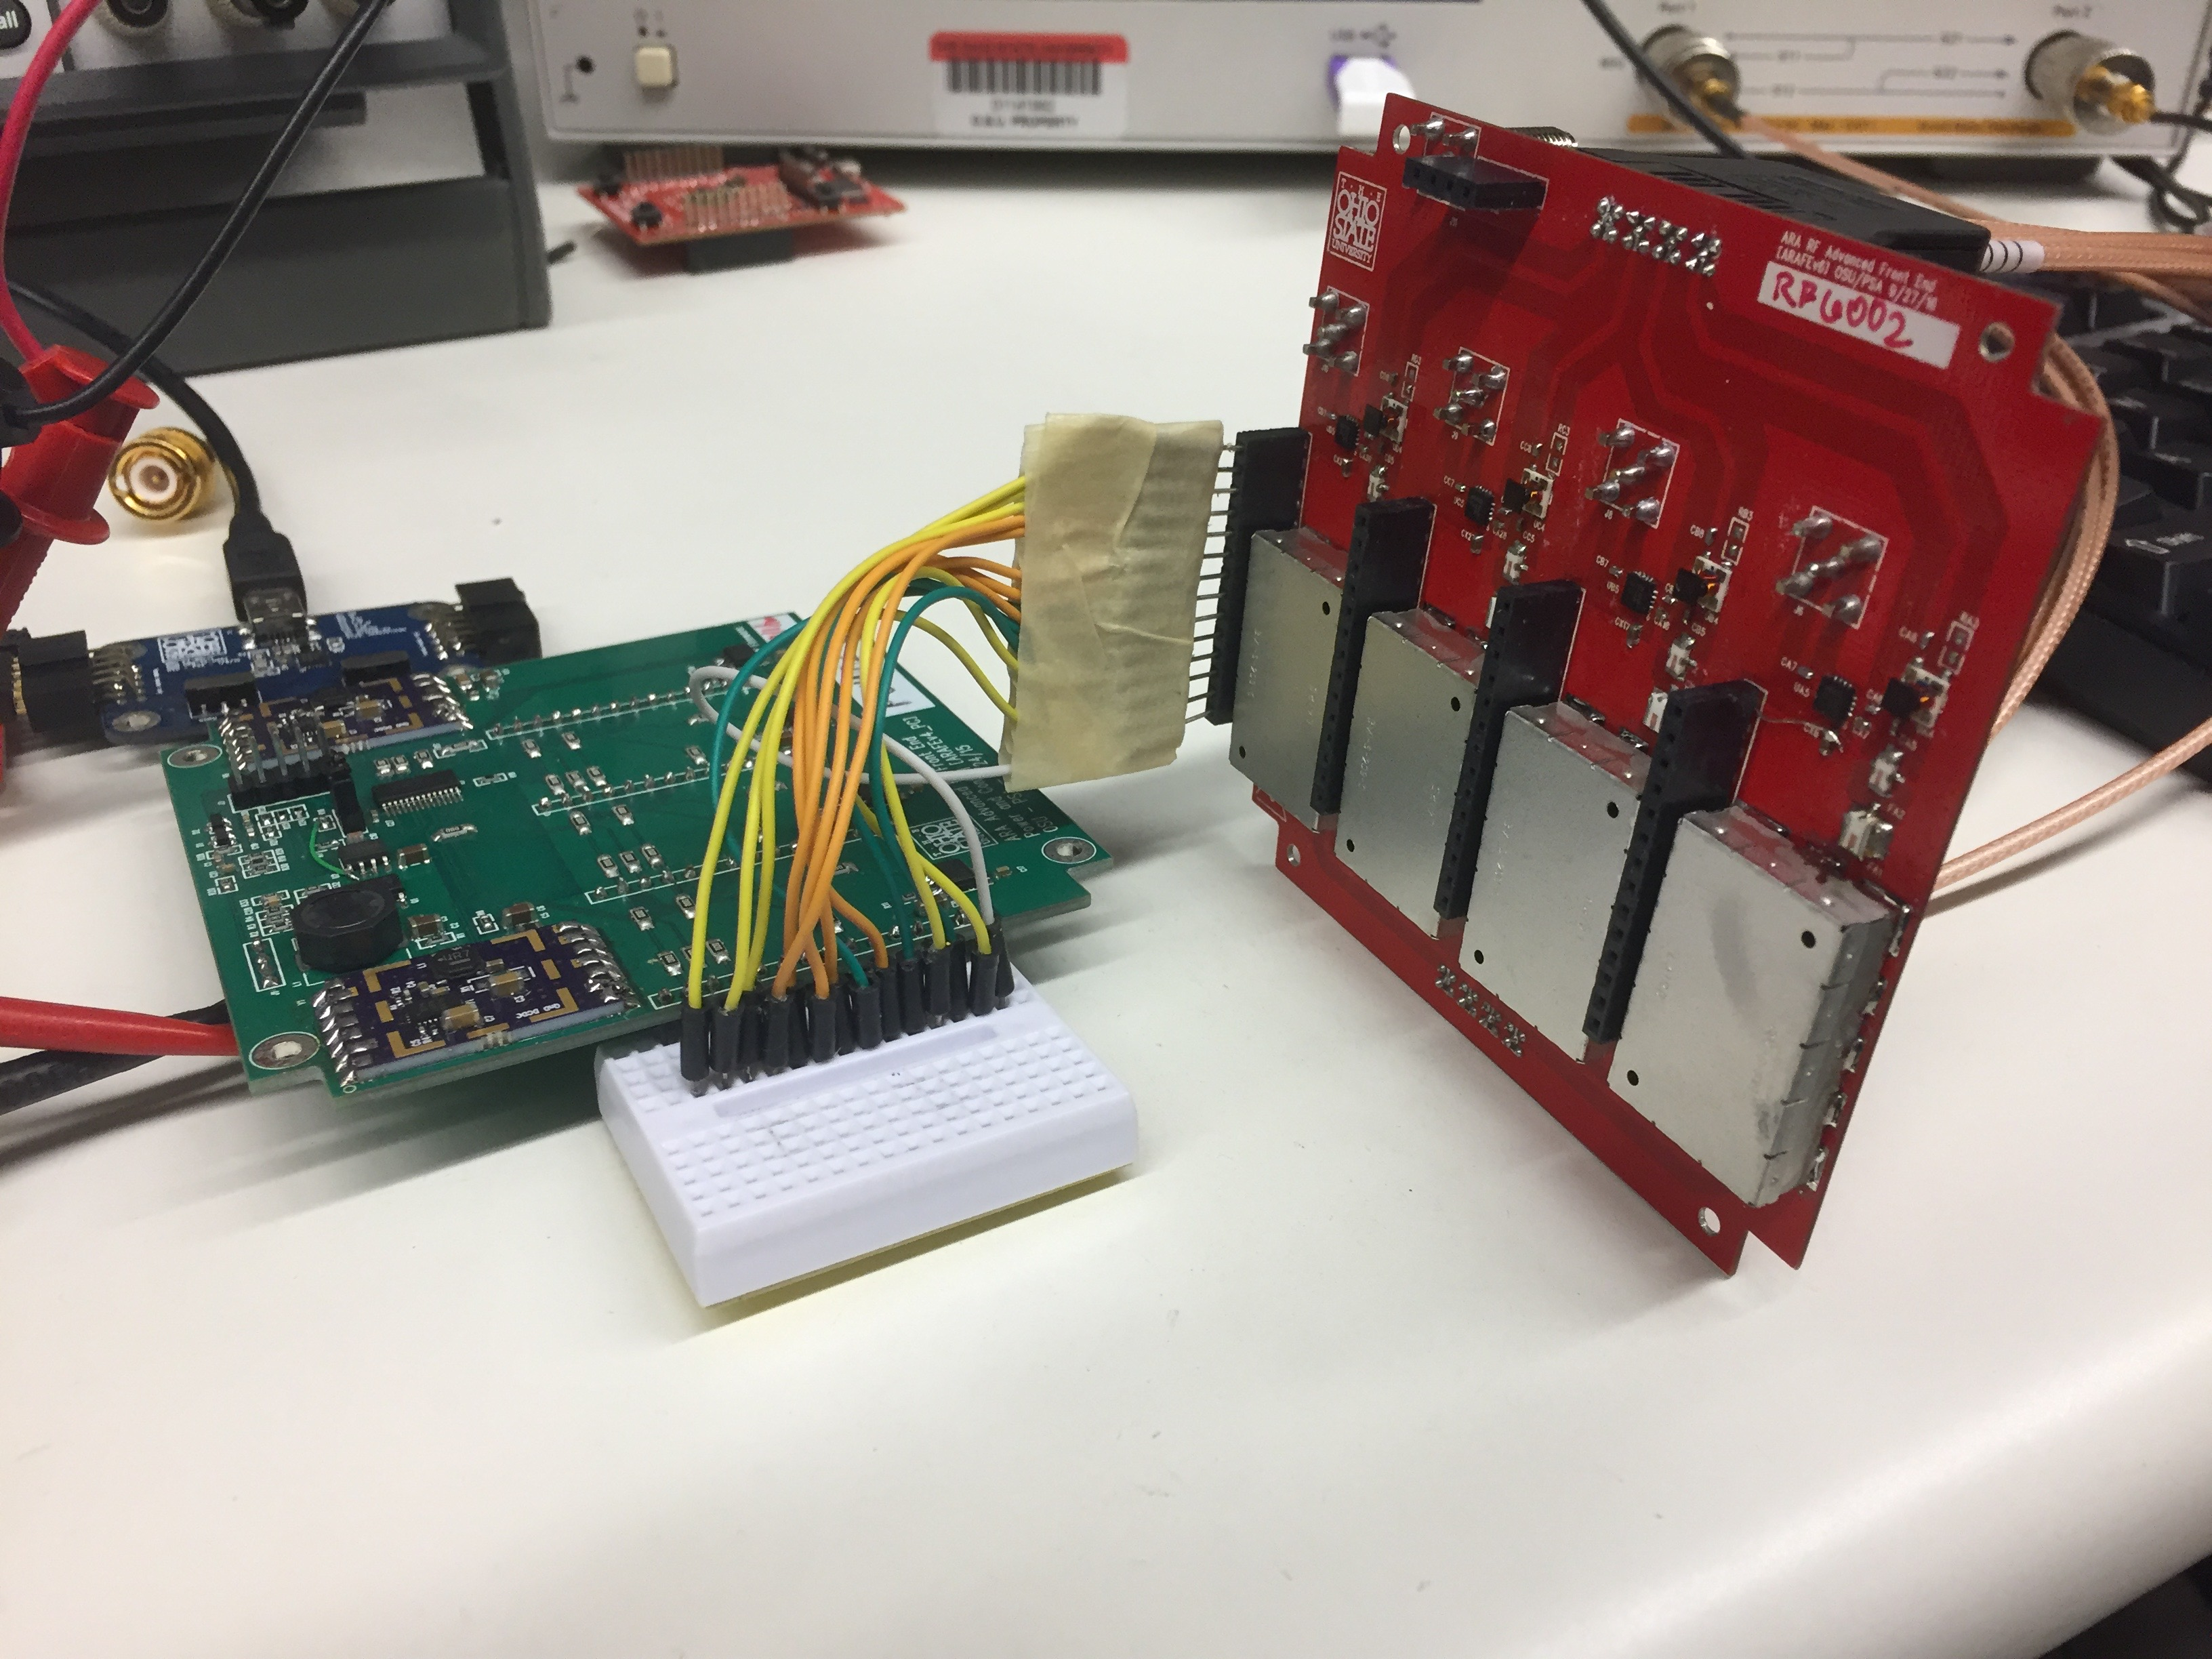
\includegraphics[width=0.5\textwidth]{photos/IMG_1214.jpg}
\par\end{centering}
\caption{Figure of ARAFE RF testing setup at OSU.}
\label{arafe-test-setup}
\end{figure}

\section{ARAFE Power and Control (PC) Board}

\subsection{Overview}

The Power and Control (PC) board provides power to the RF board as well as controls power distribution downhole. The board is equipped with under-over voltage protection, reverse bias protection, and its central brain is a MSP430G2153 microcontroller. The board contains two custom, high efficiency DCDC converters; one converter steps down the 15V from the ASPS DAQ board to 5V, and the other to 12V. The 5V converter powers the RFSA variable attenuators and amplifiers for the RF board, while the 12V converter provides downhole power to the optical zonus via bias-tee. To vet a PC board, the board should be powered, and it's 5V converter, 12V converter, and microcontroller
should be tested.

\subsection{Programming the PC Board}

Programming the PC board is done via Code Composer Studio or CCS (\href{http://www.ti.com/tool/ccstudio}{http://www.ti.com/tool/ccstudio}). The code repository for the PC board is called ``arafe\_slave\_2'' and is located in the \href{https://github.com/ara-daq-hw/arafe_slave_v2}{ARA DAQ Github}. It can be loaded into CCS using CCS's Git capability: File $\rightarrow$ Import $\rightarrow$ Git $\rightarrow$ Projects from Git.

To compile and upload the code to the microcontroller, you will use the 10-pin header on the board. If you have the \href{http://www.ti.com/tool/msp-fet430uif}{TI USB FET Programmer} you can use that directly. Plug the FET programmer into your computer, and hit Run $\rightarrow$ Debug, which should upload the code to the microcontroller. If you do not have the programmer, you can use almost any of TI's development boards as programmers also. That is explained \href{http://43oh.com/2011/11/tutorial-to-use-your-launchpad-as-a-programmer/}{here} and \href{http://www.kerrywong.com/2012/04/02/using-msp430-launchpad-as-programmer/}{here} You will jumper between the development board TEST, RESET, GND, and 3.3V to the corresponding pins on the PC board. Photos of how to do this are visible in figure \ref{programming-hookup-1} and figure \ref{programming-hookup-2}.

Because the PC board/slave firmware uses the microcontroller information memory, CCS's default programming routine has to be altered. The memory management has to be changed from ``Erase Main Memory Only'' to ``Erase Main and Information Memory.'' This can be done by doing Run $\rightarrow$ Debug Configurations $\rightarrow$ Target $\rightarrow$ MSP430x $\rightarrow$ Erase Options and select ``Erase main and information memory.'' If when you try and program the board you get the following error ``MSP430: File Loader: Verification failed: Values at address 0x1000 do not match Please verify target memory and memory map.'' This is the thing to correct.

\begin{figure}
\begin{centering}
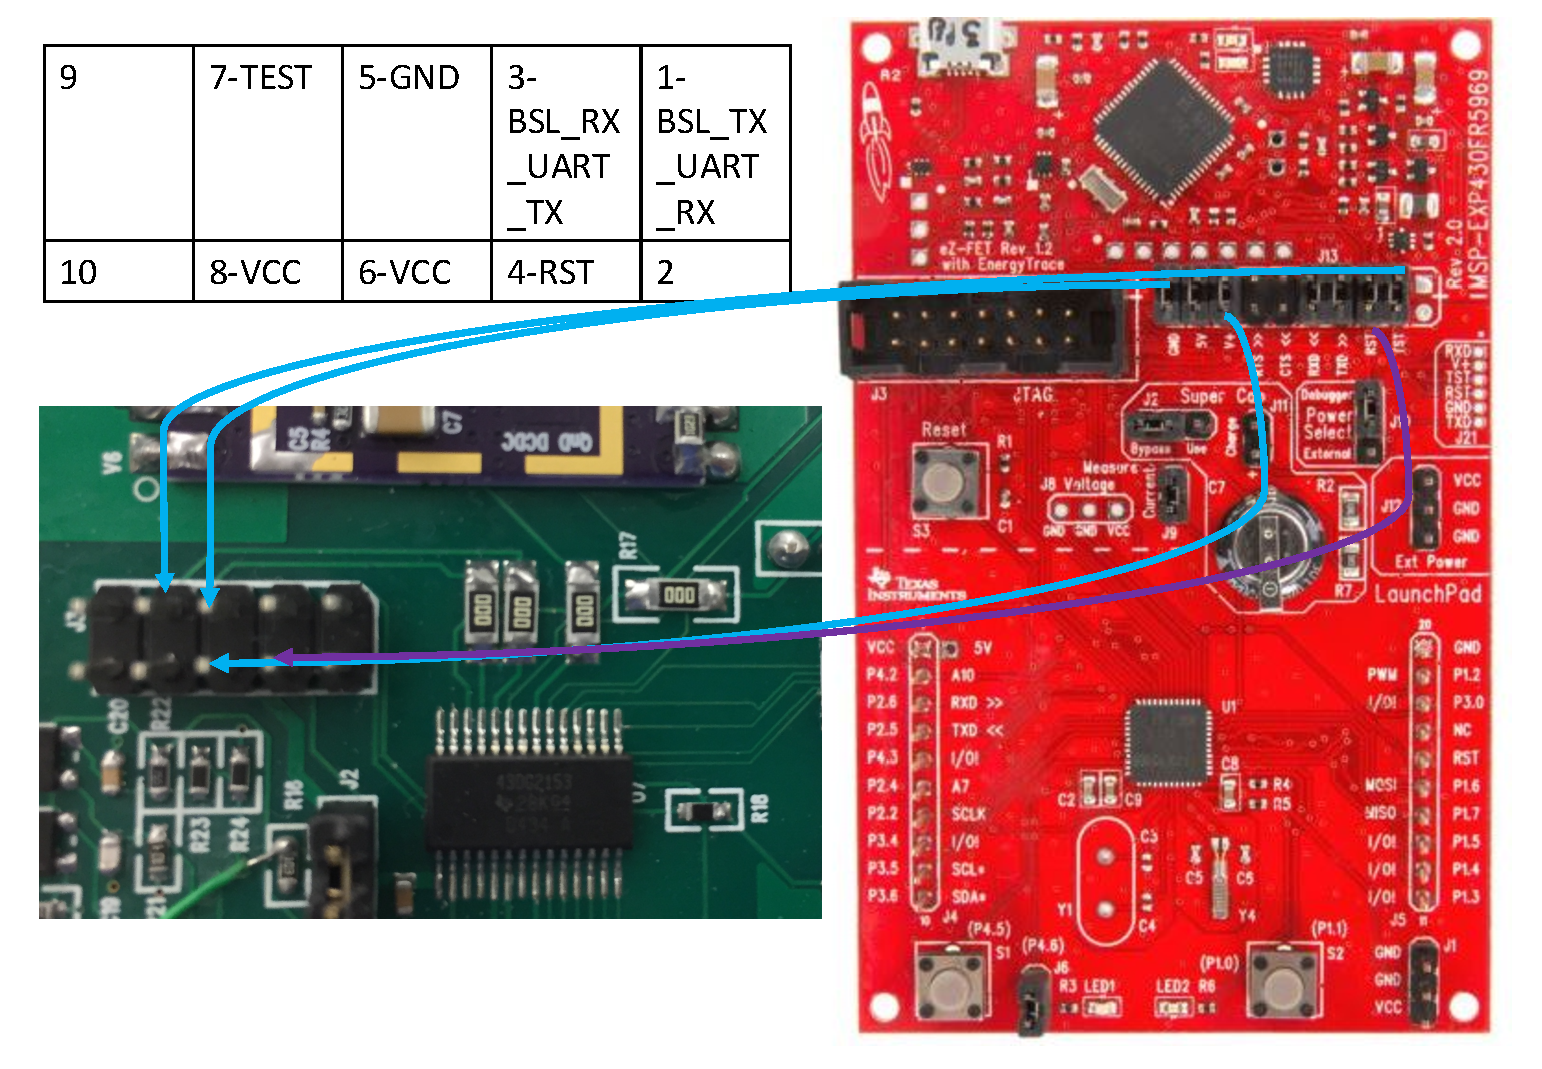
\includegraphics[width=\textwidth]{photos/programming-hookup.pdf}
\par\end{centering}
\caption{A diagram of the wire jumpering required to use a TI development board
as a programmer.}
\label{programming-hookup-1}
\end{figure}

\begin{figure}
\begin{centering}
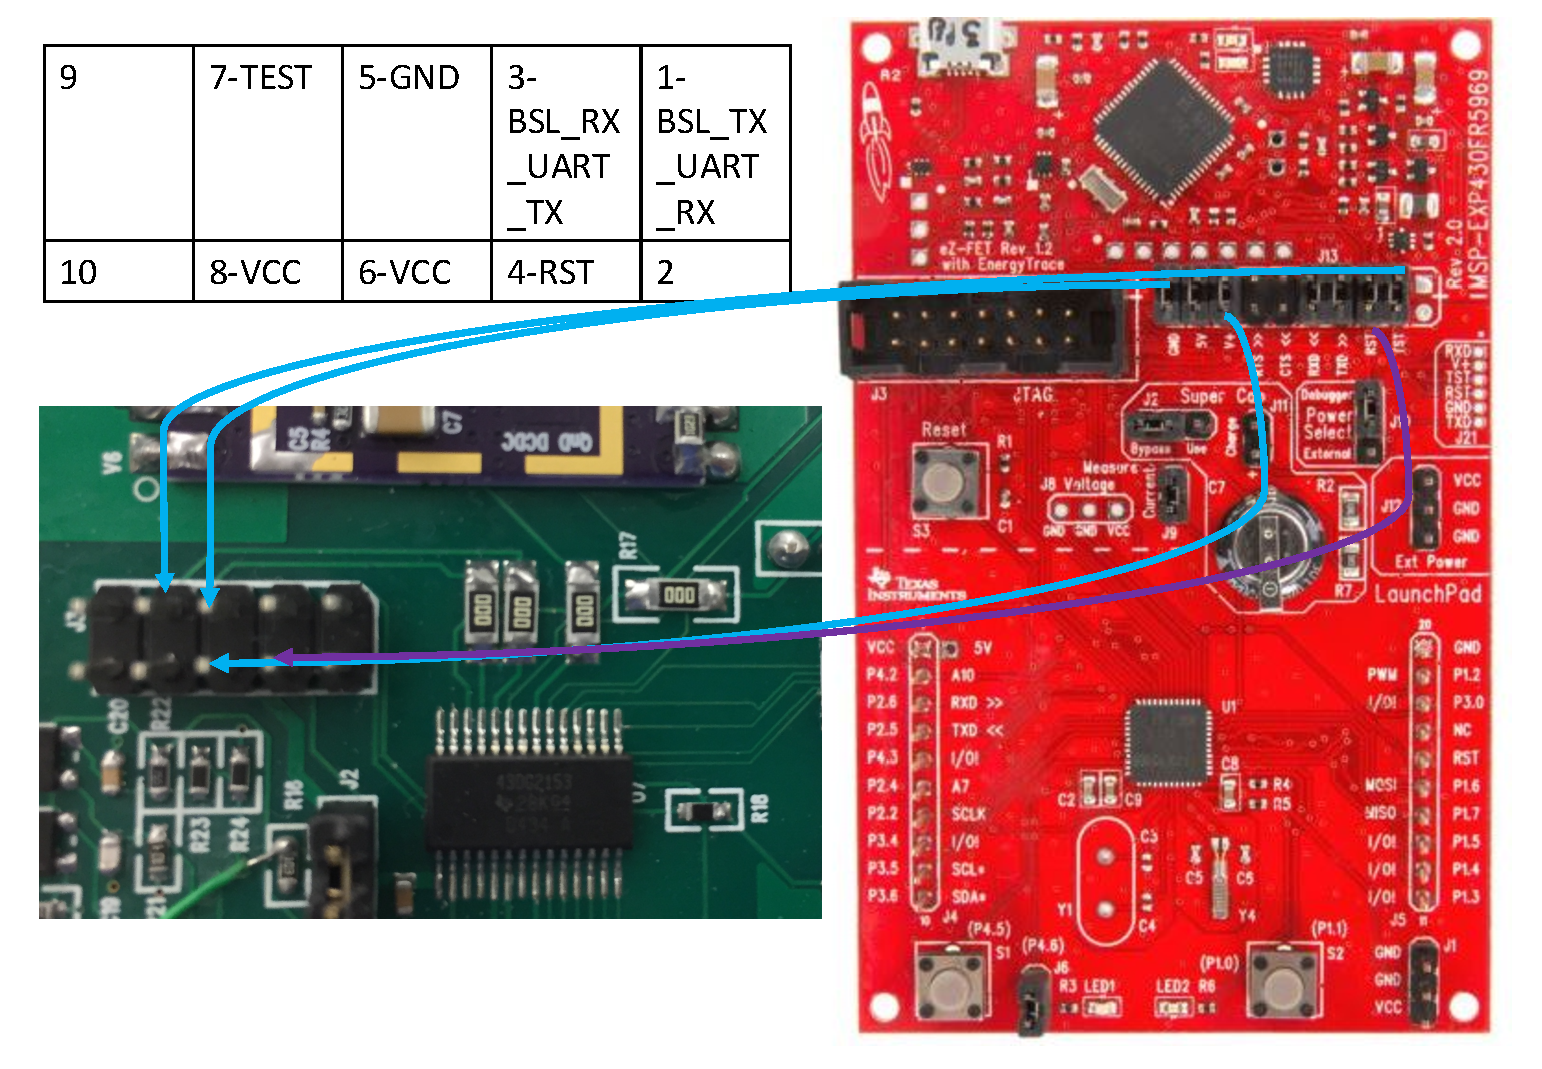
\includegraphics[width=0.5\textwidth]{photos/programming-hookup.jpg}
\par\end{centering}
\caption{A picture of programming the PC board with a TI development board
at OSU.}
\label{programming-hookup-2}
\end{figure}

\begin{figure}
\begin{centering}
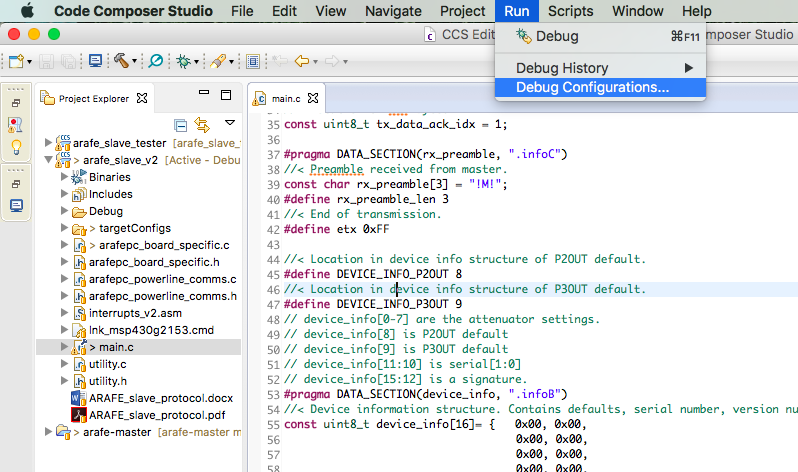
\includegraphics[width=.75\textwidth]{photos/ccs-setup-1.png}
\par\end{centering}
\caption{How to navigate to the debug configuration in CCS.}
\label{CCS-change-1}
\end{figure}

\begin{figure}
\begin{centering}
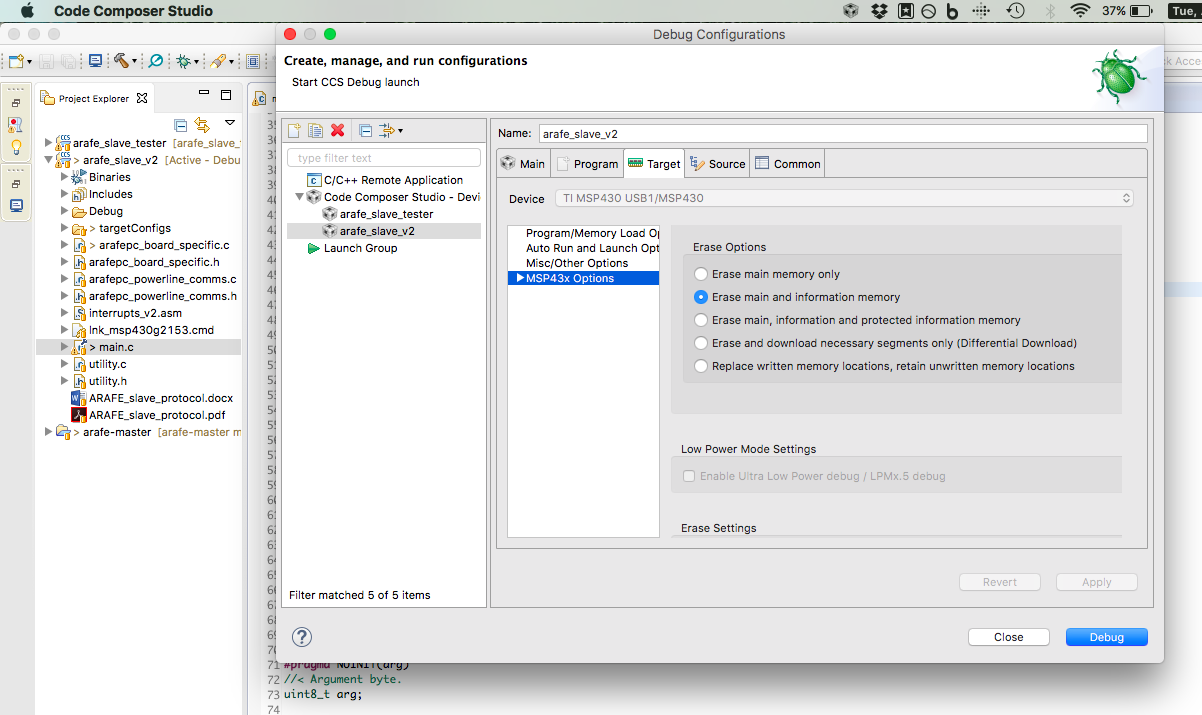
\includegraphics[width=.75\textwidth]{photos/ccs-setup-2.png}
\par\end{centering}
\caption{How to navigate to change the memory management in CCS.}
\label{CCS-change-2}
\end{figure}

\subsection{5V DCDC Converter Testing}
\begin{itemize}
\item Test the output of the 5V DCDC converter with a multimeter. It should register +5V. The output of the DCDC converter is labeled ``Vout'' in figure \ref{DCDC}.
\item Using a multimeter, probe pin 3, 8, and 14, on the jumpers, ensuring they are all +5V to begin.
\item Issue the command ``\texttt{5v 0}'' to the slave tester command line. This will turn off the 5V converter; check with the multimeter that this is true. The current drawn on the power supply should decrease. Issue the comamnd ``\texttt{5v 1}'' to re-enable the 5V converter, and ensure the multimeter registers +5V, and check that the current draw on the power supply increases again.
\end{itemize}

\begin{figure}
\begin{centering}
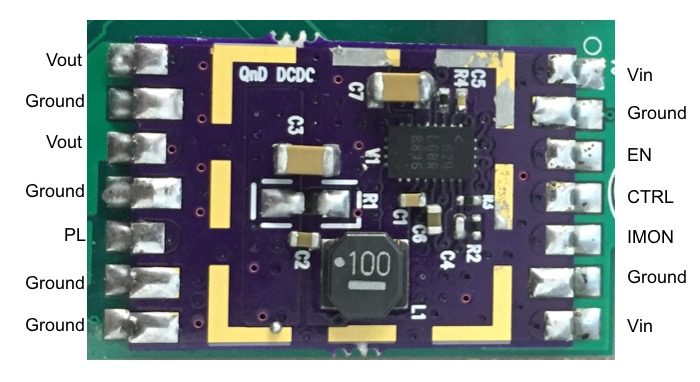
\includegraphics[width=\textwidth]{photos/DCDC.jpg}
\par\end{centering}
\caption{Photo of the DCDC converter with labeled inputs and outputs.}
\label{DCDC}
\end{figure}

\subsection{12V DCDC Converter Testing}
\begin{itemize}
\item Test the output of the 12V DCDC converter with a multimeter. It should register +12V.
\item Issue the command ``\texttt{12v 0}'' to the slave tester command line. This will turn off the 12V converter; check with the multimeter that this is true. The current drawn on the power supply should decrease. Issue the comamnd ``\texttt{12v 1}'' to re-enable the 12V converter, and ensure the multimeter registers +12V, and check that the current draw on the power supply increases again.
\item Using a multimeter, probe pin 1 of J4-J7, ensuring they are all grounded to begin.
\item Issue the command ``\texttt{control 0 [0-3]}'' to the slave tester via command line. This will enable the individual 12V lines. Probe each line (0-3) in turn with a multimeter to ensure the voltage rises to +12V. There should also be an increase in current drawn from the power supply.
\end{itemize}

\subsection{Microcontroller Testing \label{subsec:Microcontroller-Testing}}

The microcontroller job is to program the RFSA3713 variable attenuators by toggling three analog lines: CLK (clock), DATA/SI (data), and LE (latch enable). The uC also allows for some current and voltage monitoring. CLK and DATA are mutual to all attenuators on all channels. Which attenuator will ``listen'' is controlled by setting the LE pin. We want to test if the uC is issuing necessary commands, to the right attenautor, by probing each of these three pins with an oscillosope, and looking for the analog bits in the oscilloscope traces. The pin mapping between the various inputs of the attenuators, various on board jumpers, and the pin output of the uC is detailed in table \ref{PC-Jumper-RF-Mapping}.

\begin{table}
\begin{raggedright}
\begin{tabular}{|c|c|c|c|c|}
\hline 
Att Pin & Atten Function & Jumper Pin & uC Pin & uC Function\tabularnewline
\hline 
\hline 
\textbf{Ch 0} &  &  &  & \tabularnewline
\hline 
12 & Ch 0, Sig LE & JX-6 & 19 & Ch 0, Signal LE\tabularnewline
\hline 
12 & Ch 0, Trig LE & JX-12 & 18 & Ch 0, Trigger LE\tabularnewline
\hline 
13 & Ch 0, Sig and Trig Clock & JX-7 (SIG) \& JX-13 (TRG) & 27 & Global SPI Clock\tabularnewline
\hline 
14 & Ch 0, Sig and Trig Data & JX-5 (SIG) \& JX-11 (TRG) & 26 & Gobal SPI Data\tabularnewline
\hline 
 &  &  &  & \tabularnewline
\hline 
\textbf{Ch 1} &  &  &  & \tabularnewline
\hline 
12 & Ch 1, Sig LE & JX-6 & 16 & Ch 1, Signal LE\tabularnewline
\hline 
12 & Ch 1, Trig LE & JX-12 & 17 & Ch 1, Trigger LE\tabularnewline
\hline 
13 & Ch 1, Sig and Trig Clock & JX-7 (SIG) \& JX-13 (TRG) & 27 & Global SPI Clock\tabularnewline
\hline 
14 & Ch 1, Sig and Trig Data & JX-5 (SIG) \& JX-11 (TRG) & 26 & Gobal SPI Data\tabularnewline
\hline 
 &  &  &  & \tabularnewline
\textbf{Ch 2} &  &  &  & \tabularnewline
\hline 
12 & Ch 2, Sig LE & JX-6 & 13 & Chan 2, Signal LE\tabularnewline
\hline 
12 & Ch 2, Trig LE & JX-12 & 12 & Chan 2, Trigger LE\tabularnewline
\hline 
13 & Ch2, Sig and Trig Clock & JX-7 (SIG) \& JX-13 (TRG) & 27 & Global SPI Clock\tabularnewline
\hline 
14 & Ch2, Sig and Trig Data & JX-5 (SIG) \& JX-11 (TRG) & 26 & Gobal SPI Data\tabularnewline
\hline 
 &  &  &  & \tabularnewline
\hline 
\textbf{Ch 3} &  &  &  & \tabularnewline
\hline 
12 & Ch 3, Sig LE & JX-6 & 10 & Chan 3, Signal LE\tabularnewline
\hline 
12 & Ch 3, Trig LE & JX-12 & 9 & Chan 3, Trigger LE\tabularnewline
\hline 
13 & Ch 3, Sig and Trig Clock & JX-7 (SIG) \& JX-13 (TRG) & 27 & Global SPI Clock\tabularnewline
\hline 
14 & Ch 3, Sig and Trig Data & JX-5 (SIG) \& JX-11 (TRG) & 26 & Gobal SPI Data\tabularnewline
\hline 
 &  &  &  & \tabularnewline
\hline 
\end{tabular}
\par\end{raggedright}
\caption{Details of the connectivity between the RFSA pins, the jumpers on
the PC/RF board, and the uC.}
\label{PC-Jumper-RF-Mapping}
\end{table}

\begin{itemize}
\item Prepare an oscilloscope with two probes. 
\item Issue a command to control either the ``signal'' attenuator or the ``trigger'' attenuator. The command for the signal attenuator is ``\texttt{sig [channel] [setting] = sig [0-3] [0-127]}'' while the command for the trigger attenuator is ``\texttt{trig [channel] [setting] = trig [0-3] [0-127]}''.
\item Check the CLK pins (J7 and J13) for every channel. You should see 16 clock pulses on every pin, no matter the command or channel to which the command was issued. We advise setting the trigger to this pin.
\item Probe the two data pins J5 and J11 for every channel. The height of the transmitted pulse should be roughy half that of the +5V line.
\begin{itemize}
\item Should see something like the SI line on the RFSA timing diagram \ref{RFSA-timing-diagram}. A picture of the oscilloscope trace is in figure \ref{clock-and-data}.
\item There should be a high bit at the end of the bit train (A7) regardless of the command issued.
\item Bits D7-A6 should all be low, regardless of the command issued.
\item The first bits D0-D6 should be a combination of low and high, corresponding to the command issued. Note that the seven bits are exactly the number required to control the range of the RFSA; all 0's for setting zero, or minimal attenuation, and all 1's for setting 127, or maximal attenuation.
\item One should see the same command on every data pin, no matter the command or channel to which the command was issued.
\end{itemize}
\item Check the LE pins (J6 for signal and J12 for trigger) for every channel, both signal and trigger. This is where the differences between the ``sig'' and ``trig'' commands, as well as the differences between channels, is important.
\begin{itemize}
\item You should see one bit after the last clock bit (see timing diagram
\ref{RFSA-timing-diagram}). A picture of the oscilloscope trace is in figure \ref{clock-and-le}.
\item This bit should only be present in the channel to which the command was issued. That is, if you issue ``sig 1'' you should only see a bit on the signal attenuator pin of channel 1 (header pin JX-6 of channel 1), and no other. The firmware has already been debugged, so the only way this should not work is if a pin is shorted incorrectly.
\end{itemize}
\end{itemize}

\begin{figure}
\begin{centering}
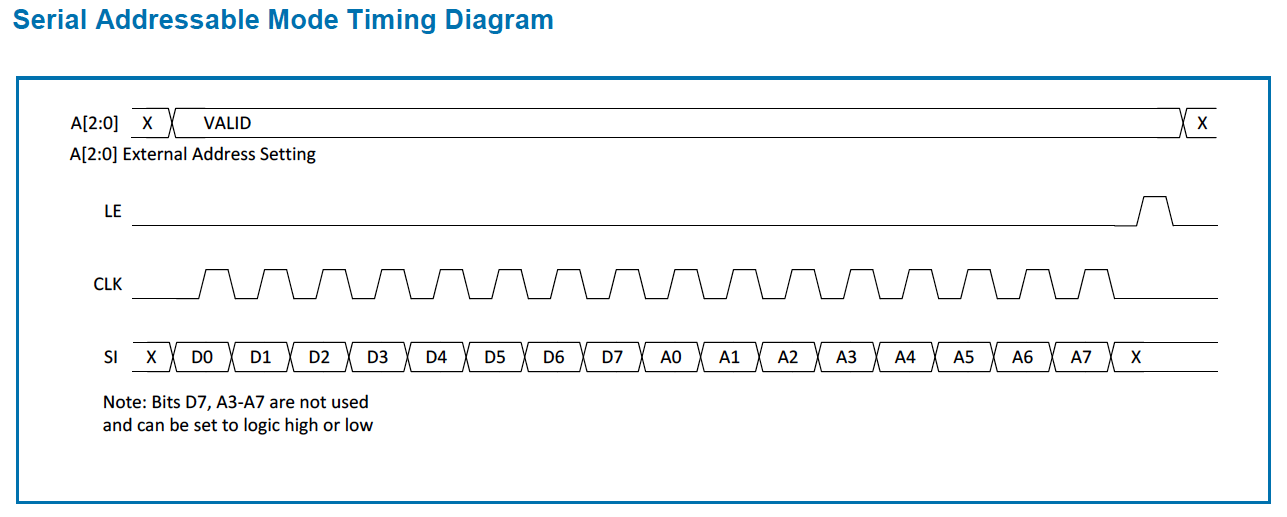
\includegraphics[width=\textwidth]{photos/RFSA-command-protocol.png}
\par\end{centering}
\caption{The bit timing diagram for programming RFSA3713 variable attenuator.
From \cite{RFSA}. }
\label{RFSA-timing-diagram}
\end{figure}

\begin{figure}
\begin{centering}
\includegraphics[width=0.75\textwidth]{photos/arafe-pc-le-on-clock.png}
\par\end{centering}
\caption{A photo of the uC clock (yellow) and latch enable (blue) pulses on
an oscilloscope.}
\label{clock-and-le}
\end{figure}

\begin{figure}
\begin{centering}
\includegraphics[width=0.75\textwidth]{photos/arafe-pc-data-on-clock.png}
\par\end{centering}
\caption{A photo of the uC clock (yellow) and data (blue) pulses on an oscilloscope.}
\label{clock-and-data}
\end{figure}

\subsection{Thermal Cycling and Programming the Serial Number in Flash Memory}

Each board should be thermal cycled, and the microcontroller test in section \ref{subsec:Microcontroller-Testing} should be repeated for all channels to check for broken soldering connections. Once it has passed it's thermal cyclce, the uC needs to be assigned the board's serial number. The uC for each PC board has onboard flash memory to store a permanent serial number. This means that the serial number can be recovered after deployment if need be. At the end of testing (post thermal cycle), a serial number should be written on the board, and flashed into memory. In revision four of the boards, for example, a PC board might have the serial number PC4002, where the ``PC'' identifies it as a power and control board, the ``4000'' identifies it as board revision 4, and the 2 is the board specific identifier. In memory, device info 10 holds the most significant byte (MSB) of the serial number, and device info 11 holds the least significant byte (LSB) of the serial number. We want the numbering to start at 4000, which is 0x0FA0 in binary. In the following example, we will program the serial number for board 4002, or 0x0FA2. So:

\begin{itemize}
\item We set the MSB to 0x0F, which in decimal is 15. So we will issue the command ``\texttt{write 10 15}''. Now, we have the total value as 0x0F00, which is 3840 in decimal.
\item Now, we set the LSB to 0xA2, which is decimal 162. So we will issue the command ``\texttt{write 11 162}''. To summarize, what we have done is program the serial number to be 0x0FA2, which is 0xF000 (3840 in decimal) + 0x00A0 (160 in decmial) + 0x0002 (2 in decimal), or 4002 total. 
\item Issue the command ``\texttt{flash}'' which will store the serial number in the flash memory of the uC.
\item Issue the dump command ``\texttt{dump}'' which will write out the content of the flash information memory to the terminal. Check that the third row, right two columns reflect the serial number you just programmed.
\end{itemize}

\section{ARAFE Radio Frequency (RF) Board}

\subsection{Construction and Initial Testing}

Testing of the RF board should be done channel by channel. After attaching surface mount components, testing of the RF channel requires installation of 

\begin{itemize}
\item an iso-rate adapter
\item a header through pin
\item an SMA.
\end{itemize}
Here is some advice on building the boards
\begin{itemize}
\item Test channel 3 first, and channel 0 last. This allows you to power up the channels, while still having full access to the surface mount components. 
\item Even without power, the S11, S22 trigger path, S22 signal path, and S21 signal path all have distinct gain patters. They can be observed in figure \ref{ideal-S11},\ref{ideal-sig-S22},\ref{ideal-trig-s22}, and\ref{ideal-sig-s21-nopwr}. Therefore, you can actually check many of the necessary connections on the board without powering it on.
\end{itemize}
Once powered:
\begin{itemize}
\item The S21 signal gain should be smooth across the band up to $\pm$2dB as in figure \ref{ideal-sig-s21-pwr}. All network analyzer traces should be from channel 2 of RF4003 (this is here for OSU's documentation sake).
\item The S21 trigger path will only be open once powered (this is because in most couplers the couple path is DC shorted to ground). The S21 gain should be as in figure \ref{idea-trig-s21-pwr}. Note:
\begin{itemize}
\item The trigger path is attenuated an additional 10 dB, consistent with the choice of coupler.
\item There are ``ripples'' in the response that are likely due to reflections off the coupler, and potentially the SMA. Given that the couple path is routed to the trigger, and the time integrator functions over \textasciitilde{}5 ns, this reflection should not affect the triggering effectiveness.
\end{itemize}
\end{itemize}

\begin{figure}
\begin{centering}
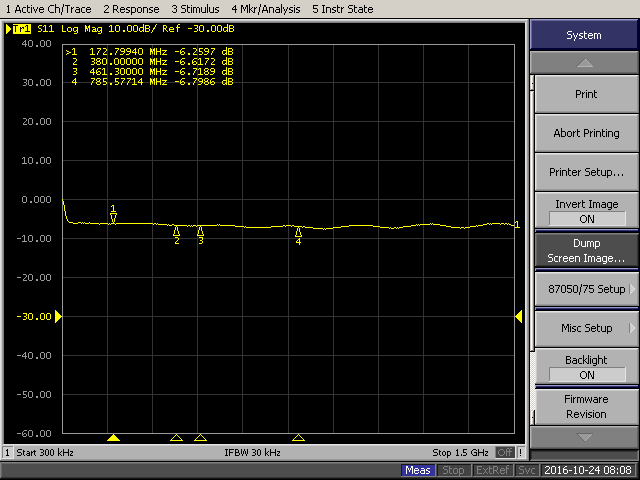
\includegraphics[width=0.75\textwidth]{photos/IDEAL-S11.PNG}
\par\end{centering}
\caption{Ideal S11.}
\label{ideal-S11}
\end{figure}

\begin{figure}
\begin{centering}
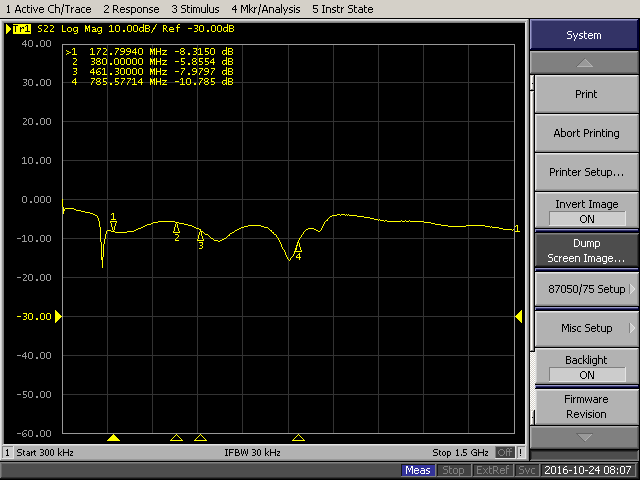
\includegraphics[width=0.75\textwidth]{photos/IDEAL-S22-SIG.PNG}
\par\end{centering}
\caption{Ideal Signal Path S22.}
\label{ideal-sig-S22}
\end{figure}

\begin{figure}
\begin{centering}
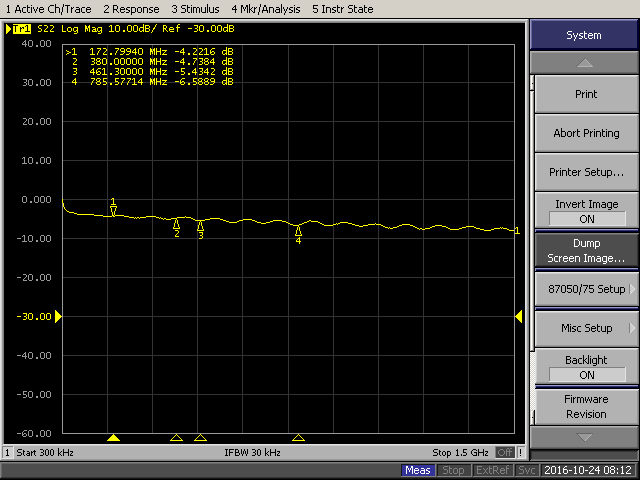
\includegraphics[width=0.75\textwidth]{photos/IDEAL-S22-TRIG.PNG}
\par\end{centering}
\caption{Ideal Trigger Path S22.}
\label{ideal-trig-s22}
\end{figure}

\begin{figure}
\begin{centering}
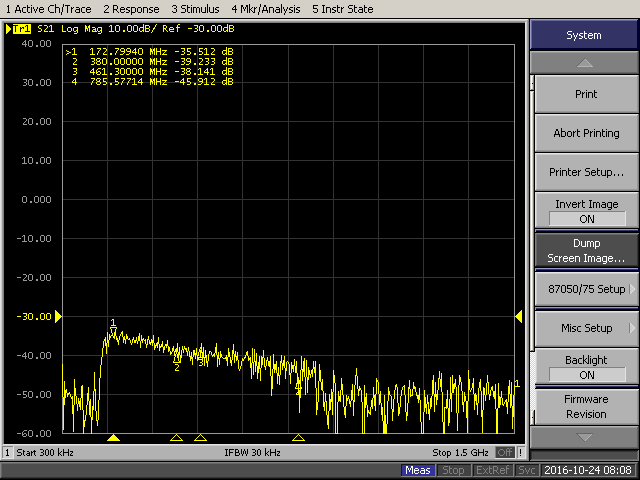
\includegraphics[width=0.75\textwidth]{photos/IDEAL-S21-SIG-NOPOWER.PNG}
\par\end{centering}
\caption{Ideal non-powered signal S21. Note that even with the power off, the
system response can be observed in the gain.}
\label{ideal-sig-s21-nopwr}
\end{figure}

\begin{figure}
\begin{centering}
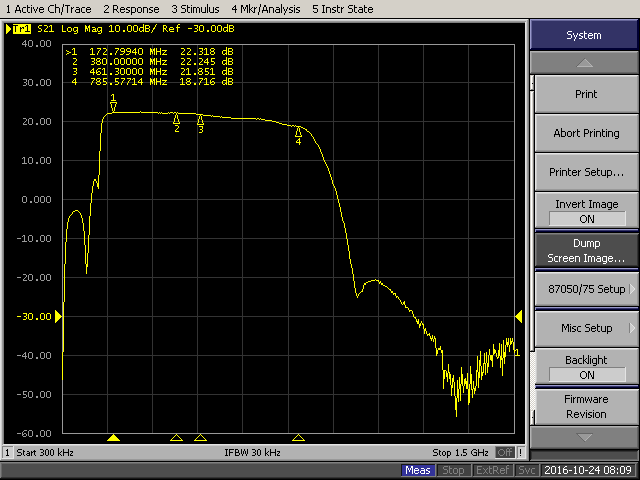
\includegraphics[width=0.75\textwidth]{photos/IDEAL-S21-SIG-POWER.PNG}
\par\end{centering}
\caption{Ideal powered signal S21.}
\label{ideal-sig-s21-pwr}
\end{figure}

\begin{figure}
\begin{centering}
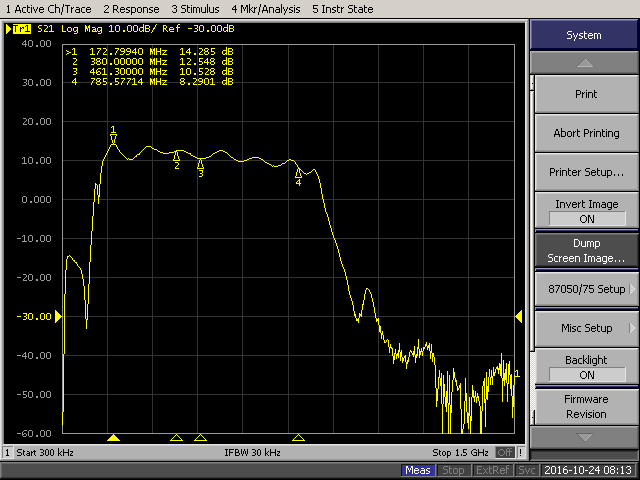
\includegraphics[width=0.75\textwidth]{photos/IDEAL-S21-TRIG-POWER.PNG}
\par\end{centering}
\caption{Ideal powered trigger S21.}
\label{idea-trig-s21-pwr}
\end{figure}

\subsection{Attenuator Testing \label{subsec:RFAttenuator-Testing}}

Now that we know the channels are working, we need to verify we can set the variable attenuators. The attenuators have a setting between 0 and 127, with each digit for a 0.25 dB increment of the 31 dB total attenuation possible with the RFSA 3713. The procedure is the following:
\begin{itemize}
\item Power a channel
\item Set the signal attenuation with the command: ``\texttt{sig [channel] [setting] = sig [0-3] [0-127]}'' Play around with various value of attenuation, and you should see the curve move up and down, as in figure \ref{sig3-example}. 
\item Set the trigger attenuation with the command: ``\texttt{trig [channel] [setting] = trig [0-3] [0-127]}''. Play around with various value of attenuation, and you should see the curve move up and down, as in figure \ref{sig3-example}.
\item In both cases, make sure that setting the attenuator to ``0'' results in minimal attenuation, and that setting the attenuator to ``127'' results in a reduction in the gain by 30 to 31 dB.
\end{itemize}
Plotted system responses for channel 3 signal and trigger paths. This was done for RF4001 (this is here for OSU's documentation sake).

\begin{figure}
\begin{centering}
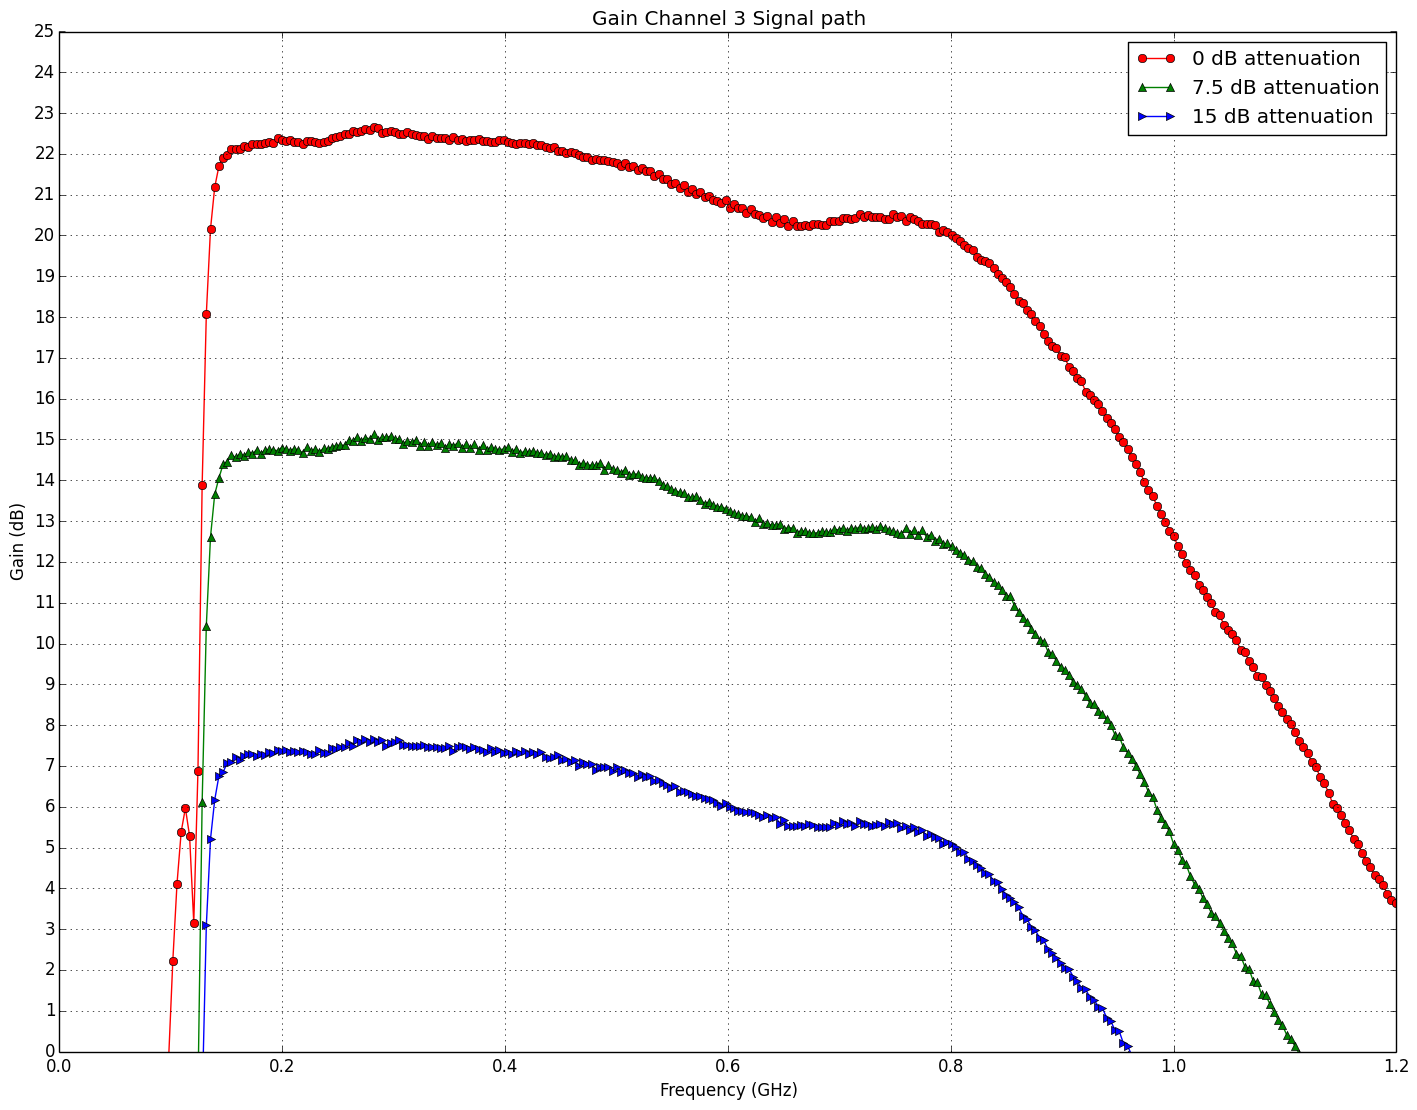
\includegraphics[width=0.75\textwidth]{photos/RF4001_SIG3.png}
\par\end{centering}
\caption{Example of a signal path gain pattern in an ARAFE at several different attenuation values. Note that this plot was made with a LFCN-800+ low pass filter. This was later replaced witha LFCN-630+ filter that has a sharper cutoff above 850 MHz. So the curve you observe should fall away more than 20 dB above \textasciitilde{}850 MHz, as in figure
\ref{sig2-example-LFCN630}. A sign that you have chosen the wrong filter is if the gain does not fall off fast enough.}
\label{sig3-example}
\end{figure}

\begin{figure}
\begin{centering}
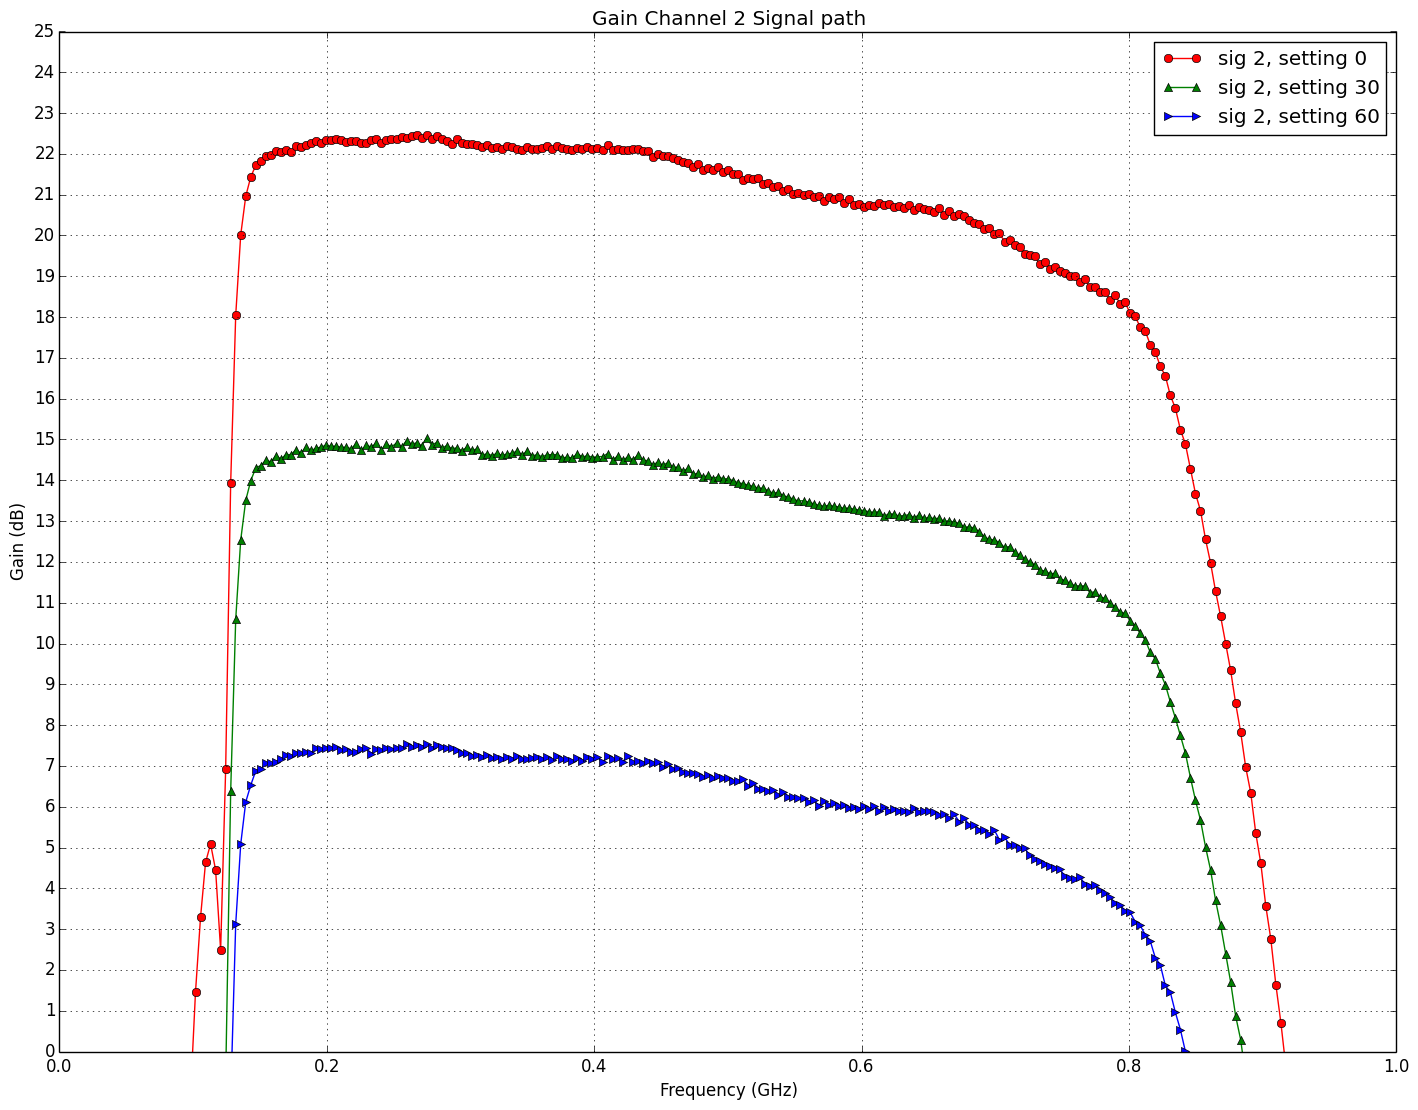
\includegraphics[width=0.75\textwidth]{photos/RF4003_SIG2.png}
\par\end{centering}
\caption{This is an example of the signal path gain with a correctly chose  filter, the LFCN-630+.}
\label{sig2-example-LFCN630}
\end{figure}

\begin{figure}
\begin{centering}
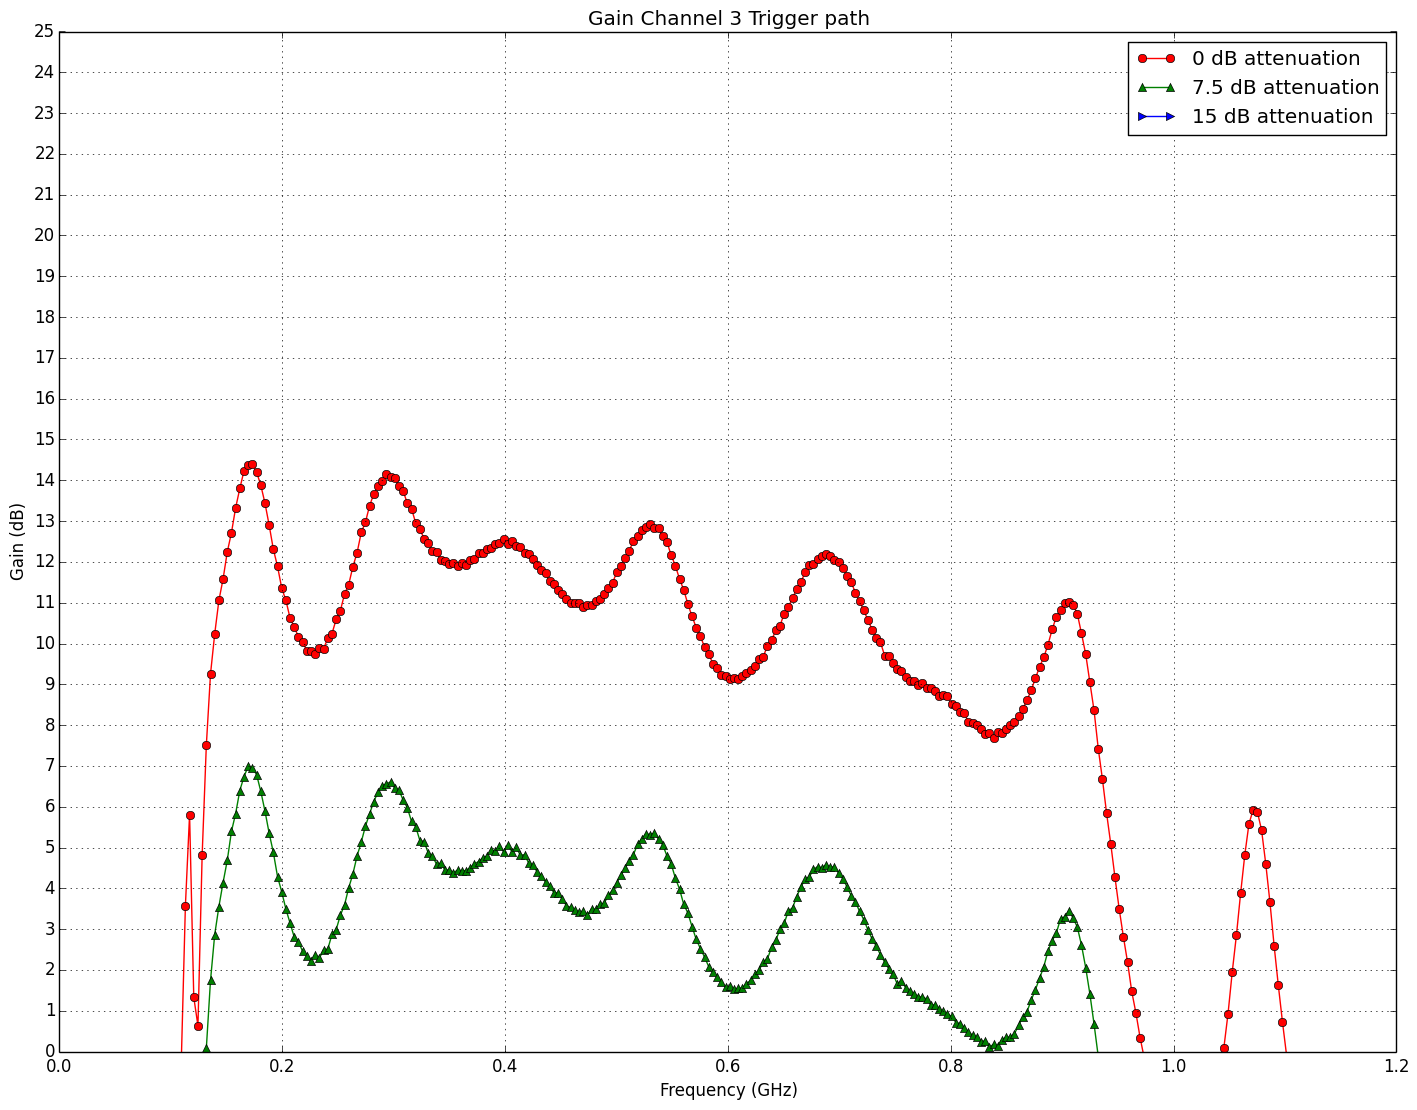
\includegraphics[width=0.75\textwidth]{photos/RF4001_TRIG3.png}
\par\end{centering}
\caption{Example of a trigger path gain pattern in an ARAFE at several different attenuation values.}
\label{trig3-example}
\end{figure}

\subsection{Thermal Cycle and RF Caging}

Once all RF channels are working, you should thermal cycle the boards, and repeat section \ref{subsec:RFAttenuator-Testing} to ensure no solder joints have broken in thermal test. If joints break, repair them. Once the boards have passed their thermal test, you should attach their RF cages, and give them a serial number on their silk screen. Attaching cages is easiest if you solder the corners first from the outside, and solder the inner pads near the headers last by poking the iron through the open cage. In all cases, you can use solder paste instead of a wire of solder if you like.

\section{RF Characterization}

\subsection{About the S-Parameters}
The RF boards must be fully characterized before final integration into the DAQ. This consists of recording the complex response (phase and magnitude) of each channel of the RF board, at a variety of temperatures and attenuator settings. We should record full 2-port s-parameter (``s2p") files in an industry standard fashion, so they can be directly imported into simulation software like Qucs studio.

 \subsubsection{File Storage}
The RF characterization files are stored in the ARA Data Warehouse at the University of Wisconsin. For ARA collaborators with Cobalt access, you can find the files at ``\texttt{/data/wipac/ARA/pre-deployment/ARAFE}".

There are two sub-directories. ``PROCESSED" and ``RAW". The RAW folder serves strictly as a back-up for the raw data from the Vector Network Analyzer. Analyzers and simulators should preferably use the PROCESSED data which contains the S2P touchstone files.

\subsubsection{File Labelling Conventions}
The full s-parameter files are uploaded as tar.gz files specifying the RF board, the channel and the temperature. So the naming convention is ``ARAFExxxxSIGnnnn.zip" and ``ARAFExxxxTRGnnnn.zip". ``xxxx" specifies the board, ``SIG" specifies the signal vs trigger path, and ``nnnn" specifies the temperature. ``nnnn" can be N20, N10, P00, P10, P20, or P30 for -20C, -10C, +0C, +20C, or +30C.

The labelling convention in the PROCESSED files is: 

``\texttt{ARAFExxxx\_SIGy\_SIGzzz\_TRGvvv\_Tnnn.s2p}".

Where ``xxxx" is the name of the ARAFE quad number, so ARAFE60002 is for RF board 6002. ``y" is the channel; so 0 means RF channel 0, 3 is RF channel 3, etc. ``zzz" is the setting of the signal attenuator from 0 to 127. ``vvv" is the trigger attenuator setting from 0 to 127. ``nnn" designated the temperature; so P00 means positive 0C,  etc.

The labelling convention in the RAW files (from the OSU Vector Network Analyzer) is 

``\texttt{ARAFExxxx\_SIGy\_SIGzzz\_TRGvvv\_Tnnn\_SmmmGDL.CSV}", 

``\texttt{ARAFExxxx\_SIGy\_SIGzzz\_TRGvvv\_Tnnn\_SmmmMAG.CSV}", 

``\texttt{ARAFExxxx\_SIGy\_SIGzzz\_TRGvvv\_Tnnn\_SmmmPHS.CSV}". 

Where ``xxxx" is the name of the ARAFE quad number, so ARAFE60002 is for RF board 6002. ``y" is the channel; so 0 means RF channel 0, 3 is RF channel 3, etc. ``zzz" is the setting of the signal attenuator from 0 to 127. ``vvv" is the trigger attenuator setting from 0 to 127. ``nnn" designated the temperature; so P00 means positive 0C,  etc. ``mmm" designates which s-parameter, so S21, S11, etc. ``GDL" designates the file as a group delay file, ``MAG" designated it as a log-magnitude file, and ``PHS" designates it as a phase file.

These are merged into the PROCESSED S2P files described above by the procedure described in section  \ref{data_processing}.
 
\subsection{Taking the S-Parameters}\label{sparams}

The procedure for characterization is as follows:
\begin{enumerate}
\item Put the quad in a thermal chamber, and let it settle at that temperature for 2 hours. We recommend six temperatures, -20C, -10C, 0C, 10C, 20C, and 30C.
\item After settling at that temperature, take the complex 2-port s-parameter file for every channel. This means you should take the magnitude and phase for S11, S22, S12, and S21.
\begin{enumerate}
\item For every signal channel, you should take the s-parameter file for the following attenuation values: 0, 8, 16, 24, 32, 40, 48, 56, 64, 72, 80, 88, 96, 104, 112, 120.
\item For every trigger channel, you should loop over the following signal settings: 0,16,32,48,64,80,96. For each signal setting, you should loop over the following trigger settings: 0, 8, 16, 24, 32, 40, 48, 56, 64, 72, 80, 88, 96, 104, 112, 120, and for each one, record the s-parameter file.
\end{enumerate}
\end{enumerate}

Note that following the above instructions, it means that for each signal path, there will be 16 s2p files. For each trigger path, there will be 112 files. This means that for each temperature, there will $128 \times 4 \, (\text{channels}) = 512$ files, and therefore, $512 \times 6 \, (\text{temperatures}) = 3,072$ files in total.

\subsection{Measurements at OSU}

\subsubsection{Procedure}

At OSU, we handle this by utilizing the Astroparticle Lab Libraries (\url{https://github.com/osu-particle-astrophysics/astroparticlelab-libraries}, contact OSU for access) which are a set of python wrapper classes that use the pyVISA, Modbus, and serial libraries. At OSU, the execution of the measurement code can be done by executing \texttt{sudo python meas\_arafe\_sparameter.py} on the Cherenkov server (which you can access through the Caesar server). It is listed in appendix \ref{code}.

The code has four important control functions for measurement devices in the Beatty-Connolly lab:
\begin{itemize}
\item Control of the Watlow F4 thermal chamber via Modbus.
\item Control of the Agilent E5062A Vector Network Analyzer (VNA) via pyVISA/GPIB
\item Control of the Agilent 34970 RF Multiplexer via pyVISA/GPIB
\item Control of the ARAFE slave tester via serial
\end{itemize}

A few important notes. In order to take full s2p files with the VNA, you would normally use the included ``Touchstone" VBA program that comes with the VNA. However, the E5062A can only call a VBA file from the GUI interface. So, to automate the taking of the s-parameters, we take the gain and phase separately, and merge them into s2p files afterward. This merging described in section \ref{data_processing}.

In order to take all four RF channels (sig or trig) at once, we use the Agilent 34970 RF mutiplexer. To remove the effects of this device on the S2P measurement, we perform a two-port calibration on the VNA.

Saving all of the associated files for all temperatures and channels at all of the attenuations described in section \ref{sparams} (including their group delays) will consume approximately 3.5GB. Because the hard drive storage on the VNA is small, we save the files to a flash drive that has sufficient storage space.


\subsubsection{Data Processing}\label{data_processing}

To merge the RAW CSV files into the compact S2P files, we use the python programs listed in appendix \label{sig_merg} and \label{trig_merg}. They are executed by running  \texttt{python sig\_merge\_csv\_to\_s2p.py} and \texttt{python trig\_merge\_csv\_to\_s2p.py}. The code uses the Pandas libraries to merge the files, and are self documenting.

\begin{thebibliography}{1}
\bibitem{RFSA}RFSA3713 Variable Attenuator Datasheet. \href{http://www.rfmd.com/store/downloads/dl/file/id/30109/rfsa3713_data_sheet.pdf}{http://www.rfmd.com/store/downloads/dl/file/id/30109/rfsa3713\_{}data\_{}sheet.pdf}
\end{thebibliography}
\appendix
\newpage
\section{Appendix: OSU Code to Take S-Parameters} \label{code}
\begin{tiny}
\lstinputlisting[language=Python]{code/meas_arafe_sparameter.py}
\end{tiny}

\newpage
\section{Appendix: Code to Merge CSV Signal Files} \label{sig_merg}
\begin{tiny}
\lstinputlisting[language=Python]{code/sig_merge_csv_to_s2p.py}
\end{tiny}

\newpage
\section{Appendix: Code to Merge CSV Trigger Files} \label{trig_merg}
\begin{tiny}
\lstinputlisting[language=Python]{code/trig_merge_csv_to_s2p.py}
\end{tiny}


\end{document}

